%%%%%%%%%%%%%%%%%%%%Tesis File%%%%%%%%%%%%%%%%%%%%%%%%%%%%%%%%%%%%%%%%%%%%%%%%%%%%%

\documentclass[12pt]{book}
\usepackage{cite}
\usepackage{amssymb}
\usepackage{amsthm}
\usepackage{amsmath}
\usepackage[pdftex]{graphicx}
\usepackage{setspace}
\usepackage{mathrsfs}
\usepackage{float}
\usepackage{pbox}
%\usepackage[linesnumbered,ruled]{algorithm2e}
\usepackage{algorithm}
\usepackage{algpseudocode}
\usepackage{setspace}
\setstretch{1.5}

\usepackage{fancyhdr}
\pagestyle{fancy}
\lhead{}
\chead{}
\rhead{}
\lfoot{}
\cfoot{\thepage}
\rfoot{}
%\usepackage{fancyhdr,floatpag}

%\pagestyle{fancy}
%\fancyhf{}% Clear page header/footer
%\renewcommand{\headrulewidth}{0pt}% No header rule
\fancyfoot[C]{\thepage}

%\floatpagestyle{fancy}% Page style for float-page only
%Theorems
\newtheorem{definition}{Definition}




%Commands

%Prior, posterior and likelihood
\newcommand{\post}{\mathbb{P}_{post}}
\newcommand{\like}{\mathbb{P}_{like}}
\newcommand{\prior}{\mathbb{P}_{prior}}
\newcommand{\p}{\mathbb{P}}
\newcommand{\q}{\textbf{q}}
\newcommand{\pars}{p,z_{0},L}
%Other commands
\newcommand{\E}{\mathbb{E}} %Expectation
\newcommand{\tvs}{\mathscr{T}} %TVS symbol
\newcommand{\x}{\textbf{x}}
\newcommand{\y}{\textbf{y}}
\newcommand{\vv}{\textbf{v}}
\newcommand{\argmax}{\mathop{\mathrm{argmax}}}
\newcommand{\argmin}{\mathop{\mathrm{argmin}}}
\newcommand{\dv}{\nabla\cdot}
\DeclareMathOperator*{\cov}{cov}
\DeclareMathOperator{\dom}{dom}
%\DeclareMathOperator{\det}{det}


\begin{document}
\setlength{\unitlength}{1 cm} %Especificar unidad de trabajo
\thispagestyle{empty}
\begin{center}
    %\begin{picture}(18,4)
    %\centering
    
\includegraphics[scale=0.5]{log.png} \\[1cm]
    %\end{picture}
\textbf{{\LARGE Simon Fraser University}\\[0.5cm]
{\LARGE Faculty of Sciences, Math Department}}\\[1.25cm]
\begin{doublespace}
{\huge \textbf{Here comes the title}}\\[1.5cm]
\end{doublespace}
{\large Juan Gabriel Garc{\'i}a Osorio}\\[1cm]
Advisor: John Stockie\\[1cm]
Commitee: Paul Tupper\\[1cm]
Burnaby B.C - May  2017
\end{center}

\newpage
\tableofcontents


%%%%%%%%%%%%%%%%%%%%%%%%%%%%%%%%Chapter 0 %%%%%%%%%%%%%%%%%%%%%%%%%%%%%%%%%%%%%%%%%%%%%%%%%%%%%%%
\chapter*{Acknowlegments}
\newpage


%%%%%%%%%%%%%%%%%%%%%%%%%%%%%%%Chapter 1: Introduction %%%%%%%%%%%%%%%%%%%%%%%%%%%%%%%%%%%%%%%%%%
\chapter{Introduction}

With the concern for climate change and anthropogenic impact on the environment, 
the importance of atmospheric dispersion models has grown over the years. Unfortunately
atmospheric disperssion model's predictions cannot be  completely accurate \cite{chatwin1982use,lewellen1989meteorological}. 
Although the precision of a model can be improved at the expense
of adding more parameters that explain the missing physics in the model, even
in this case, there is a limit in how accurate a model can be.
The reason for this, comes from the fact that uncertainty sources
are diverse and different in nature, following  \cite{rao2005uncertainty}
we have 


\begin{itemize}
\item Model uncertainty: the model does not capture all the physics.
\item Data uncertainty: experimental measurements or parameters estimation are not completely accurate.
\item Stochastic uncertainty: for example, unpredictability from the physics of the atmosphere.
\end{itemize}
This impossibility for achieving totally accurate predictions
is in contrast with the continuously growing necessity to develop
more accurate and computationally efficient atmospheric dispersion models \cite{leelHossy2014dispersion}. 

The mathematical model for atmospheric dispersion that we are 
interested is the advection-diffusion equation
for the concentration $C$ of particulate zinc. The behavior of $C$
as a function of space and time is given by 
the following partial differential equation
\begin{equation}\label{eqnModelIntro}
\frac{\partial C(\x,t)}{\partial t}+\dv(\bar{\vv}C(\x,t)+\textbf{D}\nabla C(\x,t))=\sum_{j=1}^{4}q_{j}\delta(\x-\x_{j})
\end{equation}
Here $\x=(x,y,z)\in\mathbb{R}^{3}$, $t$ is the time variable, $\bar{\vv}$  is the velocity wind field, $\textbf{D}$
is the diffusivity tensor and the right hand side of the equation is the source density. In the scenario
we are interested in modeling (see Chapter 4 for details), we have four zinc sources at known locations $\{\x_{j}\}_{j=1}^{4}$ 
with strengths $\{q_{j}\}_{j=1}^{4}$ respectively. We also mention that equation \eqref{eqnModelIntro}
depends on five different parameters, these parameters will be represent by $\Theta$.
By replacing the linear operator $\dv(\vv+\textbf{D}\nabla)$ on the LHS by $L(\Theta)$, to make the dependence explicit, we can write equation \eqref{eqnModelIntro}
more compactly as
\begin{equation}\label{eqnParamtric}
\frac{\partial C(\x,t)}{\partial t}+L(\Theta)C(\x,t)=\sum_{j=1}^{4}q_{j}\delta(\x-\x_{j}).
\end{equation}

 By knowing the concentration we can readily calculate
\begin{equation*}
\int_{R}\int_{0}^{T} C(x,y,0,t)v_{set}dtdxdy,
\end{equation*}
where $v_{set}$ is the settling velocity of zinc particles. 
The integral above represents the deposition of zinc in the region 
$R\subset\mathbb{R}^{2}$ over a $T$ units of time period.
In this work we are mainly concerned with the problem known as source inversion.
Our goal is to estimate the source strength vector (or just sources for short)
\begin{equation*}
\q:=(q_{1},q_{2},q_{3},q_{4})^{T},
\end{equation*}
given the deposition.
This problem is ill-posed\cite{enting1990inverse}.
Uncertainty in a model's prediction capabilities gets worst if the problem
is ill-posed. For example in an ill-posed model, small uncertainties
in the experimental data or parameters of the model, translate
as significant uncertainties in the output.

Despite the ill-posed nature of the problem, different
approaches have been envisioned for the source inversion
problem. Lin and Chang \cite{lin2002relative} used an air
trajectory statistical approach to estimate
the strength of different sources of volatile organic compounds
from anthropogenic origin. Stockie and Lushi \cite{lushi2010inverse} 
used a Gaussian plume approach to calculate different distribution
of zinc deposition in a lead-zinc smelter. With these results
they used  least-squares to perform the source inversion.
Skiba \cite{skiba2003method}  solved the adjoint equation
of the advection-diffusion equation and used least-squares 
with regularizer to obtain the source inversion. What
these approaches have in common is that they provide a point
estimate for the strength of the sources of interest but
no uncertainty about the estimate.

The Bayesian  framework has been used in the source inversion
problem, to obtain point estimates and the uncertainty associated 
with them. Sohn et.al \cite{sohn2002rapidly} developed an 
algorithm to obtain estimates and uncertainties for
the location and strength of pollutant sources in buildings.To do it,
they combined Bayes rule with data obtained from a simulation 
done using the software COMIS. Hosseini and Stockie \cite{hosseini2016bayesian}
used a Gaussian plume model coupled with 
experimental data and  Gaussian processes to estimate
and quantify the uncertainty of airborne fugitive
emissions in Trail, British Columbia, Canada. Using
experimental data from the transport and dispersion 
experiment ``The Muck Urban Setting Test", Keats \textit{et al}. \cite{keats2007bayesian}
obtained, using the Bayesian framework, probability distributions for sources strengths
and their locations, and used them to obtain estimates and the uncertainties associated with them.

In this work we apply the Bayesian framework  to estimate the source 
strength vector $\q$
given a set of experimental measures denote by $\y$. Unlike
the previous work mentioned above, we will also  estimate and
quantify the uncertainty in the estimates for the set of parameters $\Theta$.
This will be achieved by obtaining a joint probability
density for the parameters  and sources.  More precisely
we use Bayes rule to obtain the posterior distribution for parameters
and sources. Formally the posterior distribution can be written as
\begin{equation*}
\post(\Theta,\q|\y)=\frac{\like(\y|\Theta,\q)\prior(\Theta,\q)}{Z(\y)}.
\end{equation*}

Traditionally, the process of tuning the parameters in atmospheric dispersion models has been done
empirically based on Pasquill stability classes \cite{turner1994workbook, seinfeld1998atmospheric}.
Instead, we propose a novel approach to estimate
the parameters using the information contained in the posterior probability distribution. 
The advatange of this method is that we are taking into account the experimental data 
available, we are letting the data ``speak" about what choices of the parameters
ought to be, given the observations.

In this work we also address a method to deal with computationally expensive models.
To simulate equation \eqref{eqnModelIntro} we use a finite volume code, whose
computational overhead is high, therefore, using it several times to obtain an approximation for
the likelihood $\like(\y|\Theta,\q)$ is not feasible. Instead we ran the code 
for a small  number of different
combinations of parameters and sources ,and use an emulator based
on Gaussian process regression to extrapolate results
from the simulation to arbitrary combinations of parameters and sources. To 
reduce the computational cost even further, we performed
a sensitivity analysis that allowed us to reduce the dimensionality
of the parameter space from five to three. This reduction permitted 
us to approximate the likelihood function  and to use Markov
Chain Monte Carlo Methods to sample from the posterior faster.
We then used these samples to obtain point estimates and uncertainties
for the parameters and sources.

To conclude this chapter, we will explain how this work is organized:
in Chapter 2 we explain the theory and computations behind the
Bayesian framework, sensitivity analysis and Gaussian process regression for
emulation. In Chapter 3 we introduce more theory and combine it with the topics 
developed in the previous chapter to show how parameter estimation works
on a toy problem. Finally in 
Chapter 4 we apply everything from Chapters 2 and 3 to an
industrial case study and obtain estimates for the parameters
and the sources through sampling the posterior distribution $\post(\Theta,\q|\y)$.




%%%%%%%%%%%%%%%%%%%%%%%%%%%%%%Chapter 2: Theoretical and Computational Framework %%%%%%%%%%%%%%%%
\chapter{Theoretical and Computational Framework}
%\pdfmarkupcomment[markup=Squiggly,color=green]{what eve}{Change this shit}


The framework of Bayesian statistics is the foundation of  our approach to estimate parameters and solve 
inverse problems. Unlike frequentist statistics, in the Bayesian approach, randomness
is a measure of uncertainty or lack of information,  not a matter of frequency. Consider a statement such  as:
the probability of having life in the universe is 0.01. In the frequentist
perspective, this number is interpreted as: for every hundred planets, on average, one planet shelters life.
 In the Bayesian
perspective the number 0.01 is interpreted as a measure of how certain we are about life in the universe
given the current state of knowledge about the outer space. 
Clearly there is a big philosophical
difference between these two approaches that has a direct impact in how far reaching is each point of view 
in terms of theoretical foundations and applications  \cite{jaynes2003probability}.


%Talking about Bayes rule
At this point we mention that when we talk about uncertainty we are talking about every possible 
source of randomness  or  lack of information. That is, the use of the word uncertainty in this work
is related to either \cite{kennedy2001bayesian}
\begin{itemize}
\item Epistemic: a phenomenon might not be random but the complete lack of 
understanding of it makes us see it as random.
\item Aleatory: Inherent to the nature of the phenomenon. For 
example, this is the kind of randomness physicists believe is happening in quantum mechanics.
\end{itemize}
In real life the uncertainty associated with a  measurement or  quantity 
of interest is usually connected  with the uncertainty  of other variables involved in the problem under study. 
The Bayesian framework provides a rigorous framework to study these uncertainties, 
using whatever information is available for the underlying problem. The cornerstone of this framework
in the mathematical language is known as   Bayes' formula. Before we present it, let us 
introduce some important definitions taken from \cite{dudley2002real}.

\begin{definition}\label{dfnprobabilitytriple}
A probability space is a triple $(\Omega,\mathscr{F},\p)$, where $\Omega$ is a set called 
sample space and $\mathscr{F}$ is a collection of subsets of $\Omega$ that satisfies
\begin{enumerate}
\item $\emptyset,\Omega\in\mathscr{F}$.
\item If $A\in\mathscr{F}$ then $A^{c}\in\mathscr{F}$.
\item If $A_{1},A_{2},\ldots \in\mathscr{F}$ then $\bigcup_{i\in\mathbb{N}}A_{i}\in\mathscr{F}$.
\end{enumerate}
A  collection of sets that satisfies properties 1 to 3 is called a $\sigma-$ algebra and its elements are called
events. 
\\
The map $\p:\mathscr{F}\rightarrow [0,1]$ is called a probability measure and satisfies
\begin{enumerate}
\item $\p(\Omega)=1$.
\item If $A_{1},A_{2},\ldots \in\mathscr{F}$ are pairwise disjoint, then 
\begin{equation*}
\p\left(\bigcup_{i\in\mathbb{N}}A_{i}\right)=\sum_{i\in\mathbb{N}}\p(A_{i}).
\end{equation*}
\end{enumerate}
\end{definition}

\begin{definition}
Given a probability space $(\Omega,\mathscr{F},\p)$ and two events $A,B\in\mathscr{F}$, with $\p(B)\neq 0$,
we define the conditional probability of $A$ given $B$ by

\begin{equation*}
\p(A|B)=\frac{\p(A\cap B)}{\p(B)}.
\end{equation*}
\end{definition}


With the definitions above, we are now in position to state Bayes' fomula as
\begin{equation}\label{eqnBayes}
\post(A|B)=\frac{1}{Z}\like(B|A)\prior(A).
\end{equation}


%In equation (\ref{eqnBayes}), $\p,\prior,\like,\post$ are different probability measures defined in the
%same sample space $\Omega$. 
The sets $A$ and $B$ are subsets of the sample space $\Omega$ and 
are elements of the associated $\sigma-$algebra $\mathscr{F}$. The  notation
 $\like(\cdot|\cdot)$ or $\post(\cdot|\cdot)$, denotes conditional probability. Let us introduce some terminology:
 the term $\like(B|A)$ is called the \textit{likelihood} of $B$ given $A$. The term $\prior(A)$ is called the 
\textit{prior} probability for $A$. The prior probability expresses how much we believe the event $A$ 
to happen without assuming
anything about  $B$. The reciprocal of $Z$ is a \textit{normalization constant} defined as 

\begin{equation}\label{eqnNormalizationConstant}
Z=\int_{\Omega} \like(B|A)d\prior.
\end{equation}

The integral
is understood in the  Lebesgue sense as the  integral with respect to the measure $\prior$ \cite{lerner2014course}. 
The term $\post(A|B)$ is  the \textit{posterior} probability of $A$ given $B$. The posterior contains  the information 
that we gained by comparing our beliefs (decoded in the prior probability) with experimental data 
(decoded in the likelihood). 
\newline



%Ilustratory example
Now we look at the connection between Bayesian statistics and  the field of inverse problems. 
Inverse problems are  often concerned with finding the cause of an effect, whereas a forward
problem is concerned with finding the effect of a cause. If we have information about the 
forward problem, then we can use it to obtain information about the inverse problem. Bayes' rule
puts in a mathematical language the connection between the inverse and forward problems. 
If we consider the cause to be the
event $A$ and the effect the event $B$, then the information about the forward problem
is encoded in $\like(B|A)$. The information of the inverse problem is contained in 
$\post(A|B)$. That is why in the Bayesian framework, the posterior probability
is the $\textit{solution to an inverse problem}$.

Often, inverse problems
are ill-posed, which means
that these problems might  not satisfy one or more of the following properties \cite{lebedev2012functional}:

\begin{itemize}
\item Existence: There exists a solution for the problem.
\item Uniqueness: The problem has a unique solution.
\item Stability: Small changes in inputs result in small changes in outputs.
\end{itemize}
Any such lack of well-posedness is a serious issue. For example, if the problem under study has at least one solution
but is unstable to small perturbations, how can we assess the accuracy of the solution to 
the problem?
Therefore an statistical or non-deterministic approach is called for. As explained before, the Bayesian framework 
is useful in this context. Bayes' rule connects the inverse problem  of finding the cause
of an effect through the posterior with the forward problem of finding the effect of a cause
through the likelihood in a way that is possible to quantify the uncertainty about the solution
of the problem. Let us  clarify with an example of how the Bayesian framework can be used to solve inverse problems. 
\newline

Consider the problem of finding the launch location of a rock that impacts (and cracks) a window. 
We can start by considering the following events
\begin{align*}
& A=\text{Coordinates of the launching location}.\\
& B= \text{Coordinates of the impact location on the window}.
\end{align*}
Here we assume we know $B$, but $A$ is unknown. We can use Bayes' rule to estimate $A$ through
the posterior $\post(A|B)$. In this case
we need to find the connection between $A$ and $B$ via the forward problem, i.e. given 
the launch coordinates find the impact location. This connection is encoded in the likelihood $\like(B|A)$.
In addition we also need to set the prior probability for $A$. 
\newline



Let us explain how we could estimate the different probabilities mentioned in the previous paragraph. 
First, to find the likelihood
we need to know how the rock's impact position  in the window  is related to the launch location. 
We can use
the kinematic equations  for parabolic trajectories to get \cite{arnol2013mathematical}
\begin{equation}\label{eqnKinematics}
\textbf{r}=\textbf{r}_{0}+\textbf{v}_{0}t+\frac{1}{2}\textbf{g}t^{2},
\end{equation} 
where $\textbf{r}$ and $\textbf{r}_{0}$ are the final and initial position of the rock, 
$\textbf{v}_{0}$ is 
the initial velocity,  and $\textbf{g}$ is  a vector that points to the center of the earth and has a 
magnitude equal to the acceleration of gravity. The scalar $t$ represents time.
In a more physical language, to compute the likelihood it is necessary to estimate $\textbf{r}$ (where the 
rock hit the window) assuming we know $\textbf{r}_{0}$ (where it was thrown), and the initial velocity 
of the rock $\textbf{v}_{0}$. 
Once all the other variables are identified the value of $t$ can be computed in a straightforward manner. 

Equations in physics are just models of reality and as such are just an approximation to it. 
For example, equation \eqref{eqnKinematics} does not consider air resistance or the
Coriolis force. To take
this into account we add an extra layer to the model by adding a random parameter that accounts
for the discrepancy of our model with reality. We propose 
\begin{equation}\label{eqnParabolicEpsilon}
\textbf{r}=\textbf{r}_{0}+\textbf{v}_{0}t+\frac{1}{2}\textbf{g}t^{2}+\mathbf{\epsilon},
\end{equation} 
where $\mathbf{\epsilon}$ is a \textit{random vector} distributed as \textit{multivariate Gaussian}. 
Before we proceed it is necessary to define more terminology and mathematical objects  that are going 
to be used throughout the rest of the text. 

\begin{definition}
Given a set $\Omega$, for any subset $T\subset\Omega$, we define the $\sigma-$algebra generated by $T$ as
the smallest $\sigma-$algebra in $\Omega$ that contains $T$.
\end{definition}

\begin{definition}
Let $O$ be the set of all open sets in $\mathbb{R}^{n}$. The $\sigma-$algebra generated by $O$ is called
the Borel $\sigma-$algebra and is denoted by $\mathcal{B}^{n}$. If $n=1$ we denote 
$\mathcal{B}^{1}:=\mathcal{B}$.
\end{definition}

\begin{definition}
Given a probability space $(\Omega,\mathscr{F},\p)$, a function $X:\Omega\rightarrow\mathbb{R}$ is called 
a random variable
if $X^{-1}(C)\in\mathscr{F}$ for all $C\in\mathcal{B}$.
\end{definition}

\begin{definition}
 An $n$-dimensional random vector $\textbf{X}=(X_{1},\ldots,X_{n})$ in $(\Omega,\mathscr{F},\p)$ 
is a function $\textbf{X}:\Omega\rightarrow\mathbb{R}^{n}$ such that each component is $X_{i}$ is a random variable. 
Note that a single random variable can be considered as a one dimensional random vector.
\end{definition}

\begin{definition}
Given a probability space $(\Omega,\mathscr{F},\p)$ and an $n$-dimensional  random vector 
$\mathbf{X}:\Omega\rightarrow\mathbb{R}^{n}$, the distribution of $\mathbf{X}$
is the probability measure
\begin{equation*}
\mu:\mathcal{B}^{n}\rightarrow [0,1],
\end{equation*}
where  $\mu$ is defined by 
\begin{equation*}
\mu:=\p\circ \textbf{X}^{-1}.
\end{equation*}
\end{definition}
\begin{definition}
Given a random vector $\textbf{X}:\Omega\rightarrow\mathbb{R}^{n}$ with
probability distribution $\mu$, we say that $\mathbf{X}$ is absolutely 
continuous with respect to the Lebesgue measure if there exists a real valued, integrable function $\rho$
such that for all $C\in\mathcal{B}^{n}$ we have
\begin{equation*}
\mu(C)=\int_{C}\rho(x)dx.
\end{equation*}
We say that $\rho$ is the density function for $\mathbf{X}$.
\end{definition}
\begin{definition}\label{dfnrandonvariables}
Given an $n$ dimensional random vector $\mathbf{X}$ such that for any 
$C\in\mathcal{B}^{n}$ we have
\begin{equation}\label{eqnmultivariateGaussianDefinition}
\mu(C)=\int_{C}
\frac{1}{2\pi det(\Sigma)^{-\frac{1}{2}}}\exp\left[(\textbf{x}-\textbf{x}^{*})^{T}\Sigma^{-1}
(\textbf{x}-\textbf{x}^{*})\right]d\textbf{x},
\end{equation}
then we say
that $\textbf{X}$ has a multivariate Gaussian distribution (or just Gaussian distribution) 
with mean $\textbf{x}^{*}\in\mathbb{R}^{n}$
and covariance matrix $\Sigma$. The matrix $\Sigma$ is symmetric and positive definite. We shall write
\begin{equation}\label{eqnMultivariate}
\textbf{X}\sim \mathcal{N}(\textbf{x}^{*},\Sigma).
\end{equation}
In this case the components of $\textbf{X}$ are said to be \textit{jointly Gaussian}.
\end{definition}

We now return to equation (\ref{eqnParabolicEpsilon}), and assume $\epsilon\sim\mathcal{N}(0,\sigma^{2}I)$.
Here $I$
represents the $3\times 3$ identity matrix and $\sigma>0$ parametrizes One belief in quantifying the 
accuracy  
of equation (\ref{eqnKinematics}).  By introducing a random variable into the model
we make all variables involved  in equation (\ref{eqnKinematics})
to be  random variables; that is, we now look at the  associated stochastic equation. With this notation
we can cast equation (\ref{eqnBayes}) as  
\begin{equation}\label{eqnpostrock}
\post(\textbf{r}_{0}|\textbf{r},\textbf{v}_{0})=\frac{\like(\textbf{r}|\textbf{r}_{0},\textbf{v}_{0})
\prior(\textbf{r}_{0})}{Z},
\end{equation}
where we assumed independence between $\textbf{r}_{0}$ and $\textbf{v}_{0}$.
Since $\mathbf{\epsilon}$ is Gaussian we can readily obtain \cite{Somersalo}
\begin{equation*}
\textbf{r}|\textbf{r}_{0},\textbf{v}_{0}\sim \mathcal{N}(\textbf{r}_{0}+\textbf{v}_{0}t+\frac{1}{2}\textbf{g}t^{2}
,\sigma^{2} I).
\end{equation*}
This last equation gives an explicit density for the likelihood. 

We now turn our attention to  the prior.
Suppose that we suspect the rock was thrown from the bedroom a neighbor.
 One way to model this suspicion is to assume a prior distribution on $\textbf{r}_{0}$ as
\begin{equation*}
\textbf{r}_{0}\sim\mathscr{N}(\textbf{w},\lambda^{2} I),
\end{equation*}
where $\textbf{w}$ is the coordinate vector of the center of mass of the neighbor's bedroom and $\lambda$ represents 
One's belief the launch location is at the point $\textbf{w}$. We note that  this is only one way to model 
 prior knowledge and other forms of the prior are also possible. Finally the normalization constant
can be found as
%probabilities  are normalized, if we integrate over the whole space equation (\ref{eqnpostrock}), we get
%\begin{eqnarray*}
%1=\int_{\mathbb{R}^{3}}\post(\textbf{r}_{0}|\textbf{r},\textbf{v}_{0})d\textbf{r}_{0}\\
%=\int_{\mathbb{R}^{3}}\frac{\like(\textbf{r}|\textbf{r}_{0},\textbf{v}_{0})
%\prior(\textbf{r}_{0})}{\p(\textbf{r}|\textbf{v}_{0})}d\textbf{r}_{0}.
%\end{eqnarray*} 
%Since the denominator in the last integrand is  constant with respect to the variable of integration 
%we conclude
\begin{align*}
Z&=\int_{\mathbb{R}^{3}}\like(\textbf{r}|\textbf{r}_{0},\textbf{v}_{0})
\prior(\textbf{r}_{0})d\textbf{r}_{0}\\
&= \frac{1}{(2\pi)^{6}(\sigma\lambda)^{3}}\int_{\mathbb{R}^{3}}
\exp\left[-\frac{1}{2\sigma^{2}\lambda^{2}}
\left(\|\textbf{r}-(\textbf{r}_{0}+\textbf{v}_{0}t+\frac{1}{2}\textbf{g}t^{2})\|^{2}
+\|\textbf{r}_{0}-\textbf{w}\|^{2}\right)\right]d\textbf{r}_{0}.
\end{align*}


Having the likelihood, prior, and normalization constant allows us to compute the posterior using
Bayes' rule. With these probabilities calculated 
we can obtain  several different estimates for the value $\textbf{r}_{0}$.  
Common choices of pointwise estimates include

%
%
%For the moment assume we have the means to sample from the 
%posterior in equation (\ref{eqnpostrock}). By having samples from the posterior we can obtain
%pointwise estimates of the parameters of interest. Common choices of pointwise estimates
%include
\begin{eqnarray}\label{eqnpointestimates}
\textbf{r}_{MAP}&=&\argmax_{\textbf{r}_{0}}\post(\textbf{r}_{0}|\textbf{r},\textbf{v}_{0}) 
\qquad\text{(Maximum a posteriori),}\\
\textbf{r}_{CM}&=&\int_{\mathbb{R}^{3}}\textbf{r}_{0}\post(\textbf{r}_{0}|\textbf{r},\textbf{v}_{0})d\textbf{r}_{0}
\qquad\text{(Conditional mean)}, \\
\textbf{r}_{ML}&=&\argmax_{\textbf{r}_{0}}\post(\textbf{r}|\textbf{r}_{0},\textbf{v}_{0})
\qquad\text{(Maximum likelihood).}
\end{eqnarray} 

Each  of these estimates has its own strengths and weaknesses. If the posterior is bimodal, then the conditional
mean might point at a value with very low probability, whereas the maximum a posteriori estimate might be more 
reliable. If the posterior has no critical points then the mean might be used as a point estimate. We can 
also assess how confident we are about the point estimate. For example, if $\textbf{r}^{*}$ is our point
estimate we can calculate a number $\alpha>0$ such that

\begin{equation}\label{eqnBayesConf}
\int_{B(\textbf{r}^{*},\alpha)}\post(\textbf{r}_{0}|\textbf{r},\textbf{v}_{0})d\textbf{r}_{0}=0.95,
\end{equation}
where $B(\textbf{r}^{*},\alpha)$ is the ball centered at $\textbf{r}^{*}$ with radius $\alpha$. This 
value of $\alpha$ can be thought of as  the Bayesian version 
of the frequentist's $95\%$ confidence interval.
Another way to estimate uncertainty is by calculating the covariance matrix of $\textbf{r}$
around $\textbf{r}_{0}$ as
\begin{equation*}
\int_{\mathbb{R}^{3}}(\textbf{r}_{0}-\textbf{r}^{*})\otimes(\textbf{r}_{0}-\textbf{r}^{*})d\post.
\end{equation*}
\newline
The diagonal of this matrix  contains the variance of each coordinate of $\textbf{r}^{*}$.

Note that the posterior is a probability density and  does not necessarily have a closed form, which
can make  difficult to calculate the uncertainties we mentioned above.
Hence we need a way of extracting information from $\post$. One approach is to generate 
independent samples
from it and do a Monte Carlo integration   to obtain the different uncertainty estimates. 
How to sample from a probability 
density and do a Monte Carlo integration will be explained in Chapter 3. For the moment, we
assume it is possible to evaluate any of the point estimates and the uncertainty measures. With 
this, we can use a point estimate from equation (\ref{eqnpointestimates}) to obtain a method to infer 
the launch location of the rock and with equation \eqref{eqnBayesConf} we can estimate how confident we are
about that estimate. 
\newline


%Caveats of computing complex models
Practical problems are often substantially more challenging than in the above example. Often times we have to 
deal with further issues such as 

\begin{enumerate}
\item Uncertainties in experimental measurements.
\item Lack of sufficient information about the physics of the problem and experimental data.
\item Computational complexity of  physical models that are too expensive to evaluate.
\item Parameters that might belong to high dimensional spaces so the associated probability density is 
hard to sample from.
\item Evaluating any of the possible point estimates for the quantity of interest might computationally difficult.
\end{enumerate}
In the problem that we outlined in  Chapter 1, we have to deal with all of  the above mentioned issues.
In this chapter we are going to discuss our approach for dealling with issues 3, 4 and 5 above. We 
omit 1 and 2, since these  are intrinsic to the physics of the problem and   the methodology used 
to obtain the experimental data, and so, they are outside of our control.


%%%%Dealing with computational complexity
\section{Dealing with  the computational complexity of the physical model}
Models of physical processes can be represented in different ways.
Following O'Hagan  \cite{o2006bayesian}, we represent the  mathematical model of the physical process
 as a function
$M(\cdot)$ so that $y=M(\x)$ where $\x\in\mathbb{R}^{n}$   and $y\in\mathbb{R}$.
Mathematical models are approximations to complex physical processes. Often times these mathematical
models are expensive to compute. It is of great advantage if the complexity
of the model can be reduced. One way to do
this is by performing a sensitivity analysis on the parameters the model depends on. Roughly, we choose a
combination of different values of the parameters and then we assess the importance of each parameter in
the output. This means that we need to run the model $M(\cdot)$ for a large set 
of different combination of its parameters.
Since realistic mathematical models are typically expensive,
this implies that   the  use of   classical methods such  as correlation
ratios, FAST method, Method of Sobol', etc. 
 are not feasible (see \cite{saltelli2000sensitivity} for details). 

Here the concept of emulator as defined in \cite{o2006bayesian} 
comes into play. We 
approximate the function $M(\cdot)$, which is  expensive to evaluate,
 with a function $\widehat{M}(\cdot)$ that is cheap to evaluate. To construct such an approximation,   
we  associate a 
probability distribution with each  possible value of $M(\textbf{x})$ and for example take 
$\widehat{M}(\x)$ to be  the mean
of this distribution. We will refer to $\widehat{M}(\cdot)$ as an emulator. 
Following \cite{o2006bayesian} we expect the emulator to satisfy the conditions in 
the following definition
\begin{definition}\label{dfnEmulator}
An emulator $\widehat{M}(\cdot)$ of a function $M(\cdot)$, is a map that:
\begin{itemize}
\item At points $\{\x\}_{k=1}^{N}$  were we know the output of the mathematical model (i.e. we know 
$M(\x_{k})$ for $k=1,2,\ldots, N$)
the emulator should satisfy $\widehat{M}(\x_{k})=M(\x_{k})$.
\item For  points $\{\x_{k}^{*}\}_{k=1}^{T}$ where we don't know the output $M(\x_{k}^{*})$, the emulator should
return an estimate $\widehat{M}(\textbf{x}_{k}^{*})$ based on the distribution for $M(\textbf{x}_{k}^{*})$. 
That estimate should reflect the uncertainty associated with
the interpolation/extrapolation done at that point.
\end{itemize} 
\end{definition}


From now on in this work we are going to refer to the mathematical model or the computationally expensive
function to calculate as $M(\cdot)$, and the emulator that approximates this function  by 
$\widehat{M}(\cdot)$.
%Talking about Gaussian processes

A  popular  method to construct an emulator with the desired
extrapolation/interpolation properties is  known as a Gaussian process regression.  

\subsection{Gaussian Processes}\label{secGPs}
The conditions on the emulator $\widehat{M}(\cdot)$ imply that we need
specify a probability distribution for each point $\textbf{x}$ in the domain of the model $M(\cdot)$.
This means that  we need to work with 
 a set with high cardinality of random variables. 
When dealing with 
several random variables there is one probability density that is computationally tractable and
easy to work with: the multivariate Gaussian distribution (see Definition \ref{dfnrandonvariables}). 
The computational tractability  of the multivariate Gaussian distribution can be used as a justification
to define a Gaussian process.
\begin{definition}\label{dfnGP}
A Gaussian process (GP) is a collection of random variables $\{g(\x)\}_{\x\in A}$ for some set $A$, 
possibly uncountable,
 such that any finite subset
 $\{g(\x_{k})\}_{k=1}^{N}\subset\{g(x)\}_{\x\in A}$ for 
$\{\x_{k}\}_{k=1}^{N}\subset A$ is jointly Gaussian
\cite{rasmussen2006gaussian}. 
\end{definition}

A GP is specified by a mean function and a covariance operator or covariance kernel. 
Following  Rasmussen \cite{rasmussen2006gaussian} we define
\begin{align*}
& m(\x):=\E(g(\x)),&&\qquad\text{(Mean)}\\
& k(\x,\x'):=\E((g(\x)-m(\x))(g(\x')-m(\x')))&&\qquad\text{(Kernel)}.
\end{align*}
If $\{g(\x)\}_{\x\in A}$ is a GP with mean $m(\cdot)$ and covariance $k(\cdot,\cdot)$ we will write
\begin{equation*}
g(\x)\sim \textbf{GP}(m(\x),k(\x,\x')).
\end{equation*} 

To  understand why the notion of a GP is useful for us, recall that our goal is to create
an emulator $\widehat{M}(\cdot)$ that approximates a function $M(\cdot)$. 
For a fixed $\x\in A$, a realization of the  random variable $g(\x)$ represents
a possible value of $M(\x)$. The mean function at that point $\x$, i.e. $m(\x)$ 
represents the best prediction of the true value of $M(\x)$, so we may set
$\widehat{M}(\x)=m(\x)$. Later we will show that one way to measure the  uncertainty 
associated with that prediction is given by the quantity $k(\x,\x)$.

 

We will use GPs to fit  functions in  high dimensional euclidean spaces, so 
that we may think
of the  index set $A$ of Definition \ref{dfnGP} as a subset of $\mathbb{R}^{n}$ for some $n\geq 1$. 
\newline

The reason why  Gaussian processes are useful in practice is that  they are 
completely characterized by the mean $m(\cdot)$ and choosing a covariance kernel $k(\cdot,\cdot)$\cite{lifshits2012lectures}. 
 For example a  common covariance or kernel is the
 squared exponential (SE) function given by  
\begin{equation}\label{eqnsquareexponential}
k(\x,\x')=e^{-\frac{1}{2}\|\x-\x'\|_{2}^{2}}.
\end{equation}
We choose to use the name ``squared exponential" instead of 
Gaussian to avoid confusion with
the probability distribution.
This  covariance function tells us that if $\x$ and $\x'$ are close in the Euclidean metric 
then they are highly correlated, whereas far away points have a correlation that decays exponentially.
How to choose the covariance function depends on the kind
of regularity we want for the realizations of the GP. We will discuss this topic in
more detail later in this chapter. For reference purposes, we list 
some of the most common kernels used in practice \cite{rasmussen2006gaussian}, setting $r=\|x-x'\|_{2}$:

\begin{itemize}
\item Squared-Exponential: $k(r;\theta)=\exp\left[-\frac{1}{2}(\frac{r}{\theta})^{2}\right]$
\item Exponential: $k(r;\theta)=\exp\left[-\frac{r}{\theta}\right]$\\
\item Matern $\frac{3}{2}: k(r;\theta)=(1+\frac{\sqrt{3}r}{\theta})exp\left[-\frac{\sqrt{3}r}{\theta}\right]$.
\item Matern $\frac{5}{2}: k(r;\theta)=(1+\frac{\sqrt{5}r}{\theta}+\frac{5}{3}
(\frac{r}{\theta})^{2})\exp\left[-\frac{\sqrt{5}r}{\theta}\right]$.
\item Power-Exponential: $k(r;\theta,p)=\exp\left[-(\frac{r}{\theta})^{p}\right]$.
\end{itemize}





\subsubsection{Gaussian Processes as Distributions Over Function Spaces}

Alternatively GPs can be viewed as  measures on function spaces, and so we now discuss them in this
context following the approach of \cite{lifshits2012lectures}.
Relevant function spaces (e.g. $L^{p}$ spaces, Sobolev spaces, etc...) are 
normed vector spaces with a topology inherited from the metric induced by the norm. So
the function spaces of interest here, are topological vector spaces (TVS). 

Let $\mathscr{T}$ be a TVS and  let $\mathscr{T}^{*}$ be its topological dual. 
We will denote the action of an 
element $h\in\tvs^{*}$ over an element $z\in\tvs$ with $\langle h,z\rangle$. Moreover 
we  define a random variable taking values in $\tvs$ as a map 
\begin{equation*}
X:(\Omega,\mathscr{F},P)\longrightarrow\tvs,
\end{equation*}
that is measurable with respect to the $\sigma$-algebra generated by the open sets
of $\tvs$. This $\sigma$-algebra is known as the Borel $\sigma$-algebra for $\tvs$.
The triple $(\Omega,\mathscr{F},P)$ is a probability space as in Definition \ref{dfnprobabilitytriple}. 
We use the shorthand notation  $X\in\tvs$ whenever the random variable $X$ takes values in $\tvs$. 
For example if $\tvs=L^{2}(\mathbb{R})$,  then  $X\in L^{2}(\mathbb{R})$ means that $X$ is a measurable
map from the probability space $(\Omega,\mathscr{F},P)$ into $L^{2}(\mathbb{R})$.

We say that a random variable $X\in\tvs$ is called Gaussian if $\langle h,X\rangle$ is
a Gaussian random variable on the real line for all $h\in\tvs^{*}$. An element $a\in\tvs$ is the 
expectation of $X\in\tvs$ if 
\begin{equation*}
\E(f,X)=\langle f, a\rangle,\qquad\text{for all }f\in\tvs^{*}.
\end{equation*}
Also a linear and positive definite operator $K:\tvs^{*}\longrightarrow \tvs$ 
is called the covariance operator (the covariance
matrix in the finite dimensional case) if
\begin{equation*}
\cov(\langle f_{1},X\rangle,\langle f_{2},X\rangle)=\langle f_{1},Kf_{2}\rangle,
\end{equation*}
for all $f_{1},f_{2}\in\tvs^{*}$. Then we say that $X$ is distributed as 
$\mathcal{N}(a,K)$. It is worth mentioning
that given a covariance operator $L$ and an element $b\in\tvs$ the distribution $\mathcal{N}(b,L)$
does not always exist\cite{lifshits2013gaussian}. But if it does exist, the  Gaussian measure $\mathcal{N}(a,K)$, is completely
identified with $a$ and $K$.
\newline


%In this work we are going to be mainly concerned to work with kernels that are at least continuous
%(For example the SE kernel in equation (\ref{eqnsquareexponential}) is $C^{\infty}$). 
As an example consider the  $\tvs=C(T)$ where 
$T$ is compact subset of $\mathbb{R}^{n}$. This is the  space of real valued continuous functions 
on
$T$. This  is a Banach
space with the norm \cite{bressan1900lecture}
\begin{equation*}
\|h\|=\max_{x\in T}|h(x)|.
\end{equation*}
The dual space of $\tvs$ is given by $\tvs^{*}=\mathbb{M}(T)$ the set of signed measures defined on 
the Borel $\sigma-$ algebra of  $T$. In this 
case the duality pairing is given by 
\begin{equation*}
\langle\mu,g \rangle=\int_{T}gd\mu.
\end{equation*}
A GP,  $\{g(t)\}_{t\in T}$ (see definition \ref{dfnGP}) with mean function $m(t)$ and 
covariance kernel $k(t,t')$, can be thought of as a Gaussian measure $\mathcal{N}(m,K)$
where
\cite{lifshits2012lectures} 
\begin{align*}
\E(f)&=m\in\mathbb{C}(T), \\
(K\nu)(t)&=\int_{T}k(t,t')d\nu(t'),\qquad\text{for }\nu\in\mathbb{M}(T).
\end{align*}

The above example illustrates the connection between GPs and distributions over function spaces, and more
precisely how  is connected to Gaussian measures on function spaces. Next we will
explain how to use GPs in practice.
\newline
Assume  we have  data $\{(\textbf{x}_{i},y_{i})\}_{i=1}^{m}\subset\mathbb{R}^{n}\times\mathbb{R}$ 
 from an expensive function  $M(\cdot)$,
where $M(\textbf{x}_{i})=y_{i}$. The set $\{(\textbf{x}_{i},y_{i})\}_{i=1}^{m}$ is called
the \textit{training set}. For
simplicity we do not presume any trend in the \textit{training outputs} $\{y_{i}\}_{i=1}^{m}$. Given the training set
we would like to infer  possible values of $M(\cdot)$ on another set of points 
$\{\textbf{x}_{j}^{*}\}_{j=1}^{k}$. This set of points  is known as \textit{test set}.
For this purpose we construct an emulator $\widehat{M}(\cdot)$ (see introduction to section 2.1) by
considering the GP denoted by $\{f(\textbf{x})\}_{\x\in\dom(M)}$
 where $\dom(M)$ 
is  the domain of $M(\cdot)$.
 By
Definition \ref{dfnGP}, the random vectors
\begin{align*}
\textbf{f}&=\begin{bmatrix}f(\textbf{x}_{1}) & \ldots & f(\textbf{x}_{m}) \end{bmatrix}^{T}, \\
\textbf{f}^{*}&=\begin{bmatrix}f(\textbf{x}_{1}^{*}) & \ldots & f(\textbf{x}_{l}^{*}) \end{bmatrix}^{T},
\end{align*}
are  jointly Gaussian with
\begin{equation}\label{eqnconditional}
\begin{bmatrix}
\textbf{f} \\
\textbf{f}^{*}
\end{bmatrix}\sim\mathscr{N}\left(0,\begin{bmatrix} K(X,X) & K(X,X^{*}) \\
						    K(X^{*},X) & K(X^{*},X^{*}) \end{bmatrix}
\right),
\end{equation}	
where the zero mean reflects the assumption of no  trend in the training output $\{y_{i}\}_{i=1}^{m}$.
The element of the submatrices in the covariance matrix are given by
\begin{align*}
(K(X,X))_{ij}&=\cov(f(\x_{i}),f(\x_{j})),\\ 
(K(X,X^{*}))_{ij}&=\cov(f(\textbf{x}_{i}),f(\x_{j}^{*})),
\end{align*}
and so on.
By the requirements of Defintion \ref{dfnEmulator},
 the realization of the random vector $\textbf{f}$ is known and is equal to $[y_{1},\ldots,y_{m}]^{T}$.  
Given this vector, we want to  infer  the vector $\textbf{f}_{*}$.
This can be achieved by obtaining the distribution of $\textbf{f}_{*}|\textbf{f}$. By well known properties
of the multivariate Gaussian distribution we  obtain  \cite{lifshits2013gaussian}
\begin{equation}\label{eqnformulameancovariance}
\textbf{f}^{*}|\textbf{f}\sim\mathscr{N}(\langle\textbf{f}\rangle,\Sigma),
\end{equation}
where
\begin{align*}
\langle\textbf{f}\rangle&=K(X^{*},X)K(X,X)^{-1}\textbf{f},\\
\Sigma&=K(X^{*},X^{*})-K(X^{*},X)K(X,X)^{-1}K(X,X^{*}).
\end{align*}
Note that  if in the above equations, we only consider one  test point, $\x^{*}$, and
we take the limit as $\x^{*}$ approaches  to the training input $\x_{j}$,
 the matrix
$K(\x^{*},X)$ reduces to a vector and  converges to  $K(\x_{j},X)$. In this case, it is not hard 
to see that the mean
would be given by 
\begin{equation}\label{eqnExactPrediction}
K(\x_{j},X)K(X,X)^{-1}\textbf{f}=y_{j},
\end{equation} 
and the covariance matrix would 
reduce to an scalar  that tends to zero as $\x^{*}\rightarrow \x$. The interpretation is that 
at a training input $\x_{j}$ the prediction is exactly equal to the  corresponding training output $y_{j}$. 
For a point $\textbf{x}^{*}$ that is not part of the training set, with $95\%$ confidence we have
\begin{equation}\label{eqnConfidence}
M(\x^{*})\in [\langle f \rangle(\x^{*})-2\sigma,\langle f\rangle(\x^{*})+2\sigma],
\end{equation}
where
\begin{align*}
\langle f\rangle(\x^{*})&=K(\textbf{x}^{*},X)K(X,X)^{-1}\textbf{f}&&\text{(Mean at point $\x^{*}$)}  \\
\sigma^{2}&=K(\textbf{x}^{*},\textbf{x}^{*})-
K(\textbf{x}^{*},X)K(X,X)^{-1}K(X,\textbf{x}^{*}) &&\text{(Variance at point $\x^{*}$)}.
\end{align*}
Equations (\ref{eqnExactPrediction}) and (\ref{eqnConfidence})  show that if we define 
\begin{equation}\label{eqnDefEmulator}
\widehat{M}(\x^{*}):=\langle f\rangle(\x^{*}), 
\end{equation}
then $\widehat{M}(\cdot)$ satisfies the 
conditions for an emulator laidout in Definition \ref{dfnEmulator}.

In Figure \ref{figChp2}, it is shown an example that summarizes the discussion above.
We consider the problem of emulating the model $M(x)=\cos(2\pi x)$
having five training points. The 95\% confidence region
shows that in the training input $\x_{j}$  the variance is zero  and $\widehat{M}(\x_{j})=y_{j}$, 
as predicted by equation (\ref{eqnExactPrediction}).
\newline

The covariance kernel is the quantity that defines the mean and covariance for
the Gaussian distribution obtained when we look at finitely many random variables in 
a Gaussian Process. Therefore choosing it
is a crucial step in the fitting process. We next discuss the properties
of kernels and how to choose them depending on the data and the smooth properties we are looking
for in the emulation process. 

\subsubsection*{Covariance Kernels}
The covariance kernel cannot be any arbitrary function $k(\x,\x^{*})$. To see why, consider  the
matrix in  equation (\ref{eqnconditional}) given by
\begin{equation*}
C:=\begin{bmatrix} K(X,X) & K(X,X^{*}) \\
 K(X^{*},X) & K(X^{*},X^{*}) \end{bmatrix}.
\end{equation*}

\begin{figure}[H]
\raggedleft
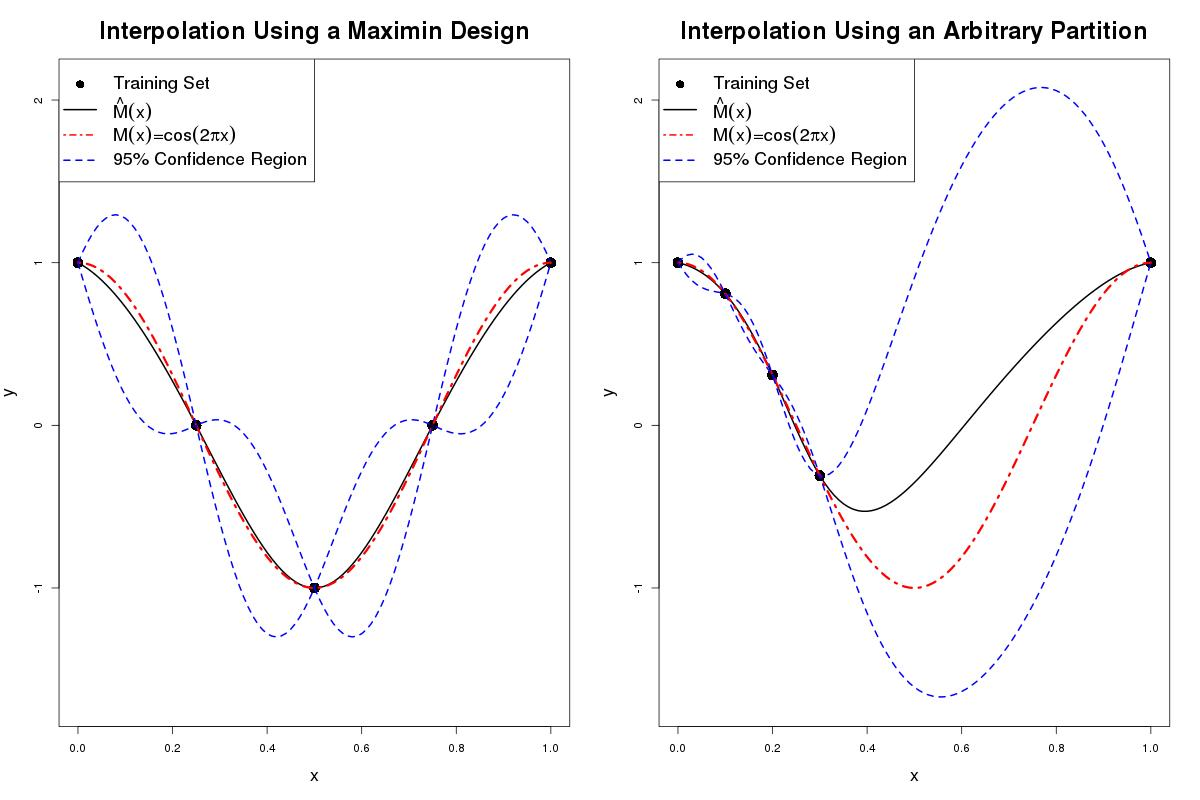
\includegraphics[scale=0.33]{./FigChap2/partitionComparison}
\caption{Comparison between the approximation quality of the emulator $\widehat{M}$ (solid line) for 
for the model $M(x):=\cos(2\pi x)$ (dashed-dotted line) in the interval $[0,1]$ for two different partitions. 
On the left, the emulation is performed in the partition $\{0,0.25,0.5,0.75,1\}$. On
the right in the partition $\{0,0.1,0.2,0.3,1\}$. The dashed line represents the $95\%$ confidence region. The
black points are the training set.}
\label{figChp2}
\end{figure}
This is the covariance matrix of a multivariate Gaussian distribution and is obtained by evaluating
the covariance kernel at different points. The matrix $C$ must be  symmetric and  positive definite 
for any set of training and test inputs. This implies that the covariance kernel has to be symmetric,
or in other words, for all $\x$ and $\x'$ in the domain of $k(\cdot,\cdot)$ we must have
\begin{equation*}
k(\x,\x')=k(\x',\x).
\end{equation*}


We also need that for  any set of inputs $\{\x_{i}\}_{i=1}^{n}$  the Gram  matrix defined by 
$K_{jk}:=k(\x_{j},\x_{k})$, must be positive definite. If  $k$ is just a function of $\x-\x'$,
which is common for many kernels of practical interest, then $k(\cdot,\cdot)$ is said to be $\textit{stationary}$.

To understand the role of the covariance kernel in the continuity and differentiability
 of the mean function, let us
define some concepts first. 
\begin{definition}
Let $\y,\x_{1},\x_{2},\ldots$ be a sequence of points in $\mathbb{R}^{n}$, such that 
\begin{equation*}
\|\x_{n}-\y\|_{2}\rightarrow 0\qquad\text{as }n\rightarrow\infty.
\end{equation*}
Then the collection of real valued random variables $\{f(\x)\}$ defined in a probability space
$(\Omega,\mathscr{F},\p)$ are said to be continuous at $y$ in the mean sense if 
\begin{equation*}
\E(|f(\x_{n})-f(\y)|^{2})\rightarrow 0\qquad\text{as } n\rightarrow\infty,
\end{equation*}
where
\begin{equation*}
\E(f(x)):=\int_{\Omega}f(x)d\p.
\end{equation*}
\end{definition}
We also have a definition for differentiability
\begin{definition}
The mean square derivative of the  collection $\{f(\x)\}$  in the $i$-th direction  at a point $\y$ is
\begin{equation*}
\frac{\partial f(\y)}{\partial x_{i}}=
\lim_{h\rightarrow 0}\E\left(\left|\frac{f(\y+h\textbf{e}_{i})-f(\y)}{h}\right|^{2}\right),
\end{equation*}
where $\textbf{e}_{i}$ is the $i$-th canonical vector of the standard basis in $\mathbb{R}^{n}$.
The mean square $n-th$ derivative is given by 
\begin{equation*}
\frac{\partial^{n} f(\y)}{\partial x_{i}^{n}}=
\lim_{h\rightarrow 0}\E\left(\left|\frac{\frac{\partial^{n-1}f(\y+h\textbf{e}_{i})}{\partial x_{i}^{n-1}}-
\frac{\partial^{n-1}f(\y)}{\partial x_{i}^{n-1}}}{h}\right|^{2}\right),
\end{equation*}
whenever the limit exists.
\end{definition}


For Gaussian processes $\{f(\x)\}$ with stationary covariance kernel, it can be shown that 
the process is continuous in the mean at a point $\y$ if and only if $k$ is continuous at $(\y,\y)$. 
Also the kernel function for the $n$-th derivative is given by \cite{adlergeometry}
\begin{equation*}
\frac{\partial^{2n}k(\x,\x')}{\partial^{2}x_{1}\ldots\partial^{2}x_{m}'}.
\end{equation*}
Therefore the continuity and differentiability properties of the mean function in a Gaussian process
depends exclusively in the continuity and differentiability properties of the covariance kernel.
\newline

Another important aspect of covariance kernels is that they are  defined in terms of parameters. 
The way we choose the values of these parameters in practice, is based on the data
we are analyzing. To see how this works, let us return to the problem of of approximating $M(\cdot)$
by $\widehat{M}(\cdot)$ using Gaussian processes. Let   $k(x,x';\theta)$ be the covariance
kernel for the GP that depends on the parameter $\theta$, where
$\theta$ could be a scalar, vector, etc. In this case to predict the output
$\y^{*}=\{M(\x_{1}^{*}),\ldots M(\x_{m}^{*})\}$ given the training set $\{(\x_{i},y_{i})\}_{i=1}^{m}$, 
we can try different approaches. One of the most common is maximum likelihood optimization (MLE), where 
we pick a parameter $\hat{\theta}$ such that
\begin{equation*}
\hat{\theta}=\argmax_{\theta}\p(\y^{*}|\{(\x_{i},y_{i})\}_{i=1}^{m},\theta).
\end{equation*}
By Definition \ref{dfnGP} we know that the conditional probability for $\y^{*}$ has to be distributed as
a multivariate Gaussian distribution. More precisely

\begin{equation}\label{eqnlikelihoodExponential}
p(\y^{*}|\{(\x_{i},y_{i})\}_{i=1}^{m},\theta)=\frac{1}{(2\pi)^{\frac{m}{2}}\det(K_{\y^{*}}(\theta))^{\frac{1}{2}}}
\exp\left[-\frac{1}{2}(\y^{*T}K_{\y^{*}}(\theta)^{-1}\y^{*})\right],
\end{equation}
where $K_{\y^{*}}(\theta)$ is the matrix $K(X,X)$ in equation (\ref{eqnconditional}). 
To find the value of $\hat{\theta}$ we have to maximize (\ref{eqnlikelihoodExponential})
with respect to $\theta$.
This goal is unchanged if we take the logarithm of  both sides and minimize the following
function instead\footnote{The reason for taking the logarithm is because most
software packages for optimization search for the minimum, not the maximum.}


\begin{equation}\label{eqnloglikelihood}
L(\theta)=-\log(p(\y^{*}|\{(\x_{i},\y_{i})\}_{i=1}^{m},\theta))=\frac{1}{2}\y^{*T}K_{\y^{*}}(\theta)^{-1}\y^{*}+
\frac{1}{2}\log|K_{\y^{*}}(\theta)|.
\end{equation}

A minimizer of $L(\theta)$   gives  a possible value for $\hat{\theta}$
that explains the best the data $\y^{*}$ given the training set $\{\x_{i},y_{i}\}_{i=1}^{m}$.  
Another common way to tune the parameters,
is using  $K$-fold cross validation, but will not use this approach here (the interested
reader is referred to \cite{murphy2012machine} for details).
\newline

So far we have not discussed  how to choose the training inputs $\{\x_{i}\}_{i=1}^{m}$. 
Clearly this choice has a profound  impact on the accuracy of the emulator.
To see this, let us assume that the function $M(\cdot)$ is supported in $[0,1]$ and we  have
computational resources to calculate the output of only five training
points. If we pick the points $\{0,0.1,0.2,0.3,1\}$ the interpolation error of the emulator
$\widehat{M}(\cdot)$  for points between $0.3$ and $1$, 
will be large, compared to the error associated with the partition $\{0,0.25,0.5,0.75,1\}$ as
shown in Figure \ref{figChp2}.
 




Ideally we would like to pick as many training points as possible to improve the fit, 
but picking too many points
to create the training set, can result in a very high computational cost. On the other hand, if we pick 
just few points to create the training set, then it is possible to end up with unreliable predictions. 
Thus we need a systematic way to choose the number and distribution of  the training points. One strategy is to  
 fill as much of the space as possible given a fixed number (possibly small) of  training points. 
This can be accomplished
through    space-filling designs which we  discuss next. 
\newline

%%%Sensitivity. The first paragraph should be relocated
\subsection{Design of Experiments }\label{secDesignofExperiments}

%Besides uncertainty there is another very important concept: sensitivity. When looking at a  model's performance
%it is critical to assess how changes or uncertainties 
% in the input $x$ affect the output $y$. Therefore if we assess sensitivity
%of the model we can assess uncertainty of the outputs. One more reason one might be interest in performing
%a sensitivity analysis is to detect what variables are relevant and what variables are not, allowing to reduce
%the dimensionality of the problem .

% To interpolate the data obtained from evaluating the computationally expensive function
%$M(\cdot)$ using GPs, we need to decide in how many different points are we going to evaluate $M(\cdot)$. 
%As mentioned in the previous section this is a very delicate issue since we need to find 
%the right balance between
%the number of possible evaluations of $M(\cdot)$ given time, computational budget 
% and a good spread of data points in the space to get a good
%fit to the model.

We assume there is a fixed computational budget. In this case, we need to decide how
to choose the training inputs $\{\x_{j}\}_{j=1}^{m}$ to obtain reliable predictions 
of the emulator for points
different than the training points. As shown in Figure \ref{figChp2}, the quality
of the emulation depends heavily on the distribution of the training inputs. 
Intuitively we want to spread the training inputs as much as possible in the
parameter space while covering  as much space as possible. 
Distributions of points that achieve this are called \textit{space filling designs}.
 
Given an set $T\subset\mathbb{R}^{n}$, there are several ways to create space filling designs. 
In this work we focus on maximin designs
\cite{johnson1990minimax}. We note that there are other ways to obtain space filling
designs and we refer to the reader to  \cite{pronzato2012design}. Consider a metric space $(T,d)$ (e.g.
$T\subset\mathbb{R}^{n}$, compact and $d$ the Euclidean distance) and a subset $S$ of $T$, 
with finite (fixed) cardinality, say $|S|=n$.
A maximin distance design $S^{o}$ is a collection of points of $T$  such that
\begin{equation*}
\max_{S\subset T,\text{ }|S|=n}\min_{s,s'\in S}d(s,s')=\min_{s,s'\in S^{o}}d(s,s')=d^{o}.
\end{equation*}
That is, we are looking for a set $S^{o}$ of cardinality $n$ that maximizes the minimum distance among 
its elements. As an example consider $T=[0,1]^{3}$, the unit cube in $\mathbb{R}^{3}$ and $n=8$. In 
this case the design that maximizes the minimum distance among its elements is given by choosing
 the 8 vertices of the cube. Or as shown if Figure \ref{figChp2} (right), if $T=[0,1]$ and $n=5$, 
the maximin design is given by a uniform partition  of the set $T$.


The problem of finding
the optimal  maximin design is difficult to solve in general. In practice we use computational tools
to find a design that is close to optimal.  Different  algorithms can be used for the optimization
of the design, such as genetic algorithms, simulated annealing, particle swarm, etc. A survey
on the subject  can be found in 
\cite{viana2010algorithm}. In Chapter 4 we will see how  the particle swarm algorithm can be used to 
create a maximin design for a five dimensional parameter space.

To conclude this section, we note that there is a conection between maximin designs and Gaussian processes. 
Consider a
GP $\{f(x)\}_{x\in T}$, fix $S=\{s_{1},\ldots,s_{n}\}\subset T$,  and consider the random vector
\begin{equation*}
\textbf{f}=[f(s_{1}),\ldots,f(s_{n})],
\end{equation*}
where $\textbf{f}$ is assumed to be jointly Gaussian. Let $K_{s}$ be 
the correlation matrix for the probability distribution of $\textbf{f}$. Then it can be shown
that the minimax design minimizes the quantity 
\begin{equation*}
D(S)=-\det(K_{s}),
\end{equation*}
where the matrix $K_{s}$ is the same as the covariance matrix in equation (\ref{eqnconditional}).
A survey of the theory behind maximin distance designs can be found in \cite{johnson1990minimax}.
\newline


%ince the covariance matrix is positive definite (hence the correlation matrix is also positive definite)
%, then $det(K_{s})>0$. By minimizing the  negative of the determinant  we are maximizing
% the determinant. This is achieved when the column vectors of a matrix
%are orthogonal. 


\subsection{Sensitivity Analysis}\label{subsecSensitivity}


Having an space filling design for the training input permits us to create an
emulator $\widehat{M}(\cdot)$ that closely approximates $M(\cdot)$  over its whole domain. 
By ``closely" we mean within a tolerable uncertainty in the output of the emulator 
for all points in the domain (see Figure \ref{figChp2}).
%Let us suppose that we have a good space filling design, we can construct a good GP, in the sense that 
%the uncertainty in the interpolation is less compared to the interpolation error when
%using other space filling design. 
%then we have a good fit when using gps to interpolate  the 
%points we want to get information about. 
If we have a reliable fitting, then we can confidently assess what parameters in the model $M(\cdot)$
are relevant and which ones are not.
This ultimately allows to approximate  the model  with a simpler one.
For example, if our model is given by 
\begin{equation*}
M(x_{1},x_{2},x_{3})=x_{1}+x_{2}+10^{-8}x_{3},\qquad(x_{1},x_{2},x_{3})\in  T=[0,1]^{3},
\end{equation*}
then clearly the variable $x_{3}$ is not as relevant as $x_{1}$ or  $x_{2}$. We need to
formalize in what sense $x_{3}$ is irrelevant. One way to achieve this is by doing a 
sensitivity analysis. In summary, the goal of a
sensitivity analysis is to assess how
the output of a function $M(\cdot)$ depends on variations of its arguments. There is
a great number of methods to perform a sensitivity analysis, such as adjoint methods, local
methods, and variance based methods, to name a few. The primary difference between each of these
methods is how they measure the importance of each variable. For example, in local methods
the sensitivity at a point in a given direction is the slope of the function, whereas in
variance based methods what matters is the magnitude of the area under the curve when
fixing all parameters but one.
For a survey of techniques in sensitivity analysis, 
the reader is referred to \cite{saltelli2000sensitivity}. 

In this work we  use 
variance-based Monte Carlo methods (VBMCM) as described in \cite{sobol1993sensitivity}.
The idea of  VBMCMs is to use the variance produced by  the inputs of a function as an indicator of 
their importance. More precisely we will use the method of Sobol', which we outline next


The functions of interest in this work have compact support. This implies that
without loss of generality we may assume that  the domain of these functions 
is the $n$-dimensional unit cube $\Omega^{n}$. Let us consider a generic
square integrable function
\begin{equation*}
\varphi:\Omega^{n}\rightarrow\mathbb{R},
\end{equation*}
and start by decomposing $\varphi$ as 
\begin{equation*}
\varphi(x_{1},\ldots,x_{n})=\varphi_{0}+\sum_{k=1}^{n}\varphi_{k}(x_{k})+
\sum_{1\leq k< l\leq n}\varphi_{kl}(x_{k},x_{l})+\ldots+
\varphi_{1,2,\ldots,n}(x_{1},\ldots,x_{n}).
\end{equation*}
This decomposition is not unique, but it can be shown that if each term $\varphi_{i_{1},\ldots,i_{j}}$
in the expansion satisfies

\begin{equation}\label{eqnSobolCond1}
\int_{[0,1]}\varphi_{i_{1},\ldots,i_{j}}dx_{i_{k}}=0\qquad\text{if }  i_{k}\in \{i_{1},\ldots,i_{j}\},
\end{equation}
then the decomposition is unique and all terms in the expansion are orthogonal in $L^{2}(\Omega^{k})$. To 
demonstrate  the orthogonality property, 
we may  consider the functions $g=\varphi_{i_{1},\ldots,i_{j}}$ and $h=\varphi_{ell_{1},\ldots,ell_{k}}$ 
with arbitrary indices $(i_{1},\ldots,i_{j})\neq(\ell_{i},\ldots,\ell_{k})$. Without 
loss of generality we may  assume $i_{1}\neq \ell_{1}$. In this case we have
%by Fubinni's theorem \cite{lerner2014course} we may conclude that functions with different subindices are 
% pairwise orthogonal in $\Omega^{n}$ with the standard inner product of $\mathbb{R}^{n}$\cite{bressan1900lecture}. 
%To see this, without loss of generality
%we may  consider the functions $g=\varphi_{i_{1},\ldots,i_{j}}$ and $h=\varphi_{l_{1},\ldots,l_{k}}$ 
%with $(i_{1},\ldots,i_{j})\neq(l_{i},\ldots,l_{k})$, with $i_{1}\neq l_{1}$. In this case we have
\begin{equation*}
\langle g,h\rangle=\int_{[0,1]}\ldots\int_{[0,1]}\underbrace{\left(\int_{[0,1]}\varphi_{i_{1},
\ldots,i_{j}}dx_{i_{1}}\right)}_{\text{$=0$ by (\ref{eqnSobolCond1})}}
\left(\int_{[0,1]}\varphi_{l_{1},\ldots,l_{k}}dx_{l_{1}}\right)dx_{\sim i_{1},l_{1}}=0,
\end{equation*}
where we used Fubinni's theorem to split the integrals \cite{lerner2014course}. The symbols to the right of $\sim$ 
represent the variables omitted in the integration.
Another consequence of  (\ref{eqnSobolCond1}) is 
\begin{eqnarray*}
\int_{\Omega^{n}}\varphi dx=\varphi_{0}.
\end{eqnarray*}
This allows us to find  the other functions in the decomposition recursively,
given $\varphi_{0}$. For example, 
for $i\in \{1,\ldots,n\}$ we have
\begin{equation*}
\varphi_{i}(x_{i})=-\varphi_{0}+\int_{[0,1]^{n-1}}\varphi(x)dx_{\sim i}.
\end{equation*}
Having $\varphi_{i}(x_{i})$ we can then proceed to find $\varphi_{ij}(x_{i},x_{j})$ using
\begin{equation*}
\varphi_{ij}(x_{i},x_{j})=-\varphi_{0}-\varphi_{i}(x_{i})-\varphi_{j}(x_{j})+
\int_{\Omega^{n-2}}\varphi(x)dx_{\sim ij}.
\end{equation*}

By knowing all of
the functions in the decomposition of $\varphi$ we are able  to assess how each variable 
affects the output of $\varphi$ in the following way. The total variance $D$ of $\varphi$ is defined as
\begin{equation*}
D=\int_{\Omega^{n}}\varphi^{2}(x)dx-\varphi_{0}^{2},
\end{equation*}
and similarly we can compute the partial variances as
\begin{equation*}
D_{i_{1},\ldots,i_{s}}=\int_{[0,1]^{n-1}}\varphi^{2}_{i_{1},\ldots,i_{s}}dx_{i_{1}}\ldots dx_{i_{s}}.
\end{equation*}
With these variances we define the $s$-th order  Sobol index  
\begin{equation*} 
S_{i_{1},\ldots,i_{s}}=\frac{D_{i_{1},\ldots,i_{s}}}{D},
\end{equation*}
which is a measure of the contribution of the variables $x_{i_{1}},\ldots,x_{i_{s}}$ to the total variance $D$.
If we want to know the separate effect  of each variable
$x_{1},\ldots,x_{n}$ in the total variance $D$, we look at
the first order Sobol indices $S_{1},\ldots,S_{n}$ given by
\begin{equation*}
S_{i}=\frac{D_{i}}{D},\qquad\text{for }i=1,\ldots,n.
\end{equation*}

Finally if we want to assess the full effect of a  variable  in the total variance $D$, 
we calculate a quantity known 
as the total effect index. For example if we want to calculate the total effect index
for the variable $x_{i}$ we would do so by calculating
\begin{equation*}
S_{i}+S_{i1}+S_{i2}+\ldots+S_{i12}+S_{i13}+\ldots+S_{12\ldots,i,\ldots, n}.
\end{equation*}

Note that  to calculate each  Sobol' index, it is necessary to perform 
high dimensional integrals. Therefore integration using quadratures is not feasible.
It is necessary to resort to other numerical integration techniques. A common
tool to perform high dimensional integrals is known as Monte Carlo integration. We will not
go into details of Monte Carlo integration in this chapter, but rather postpone them for Chapter 3.
What is important at this time is that to apply Monte Carlo integration, it is necessary to 
evaluate the integrand a large number of times at different points in its domain. If the 
integrand is the expensive model $M(\cdot)$, then the computational cost of estimating
the Sobol' indices is prohibitive. If instead we calculate the Sobol' indices 
of the emulator $\widehat{M}(\cdot)$, we can use them as an approximation for the Sobol'
indices of $M(\cdot)$. In this way we can estimate what arguments of the model are 
relevant and what arguments are not. This will allow us to reduce the complexity of the
model.

In the next chapter we will show how  the theory explained in  this chapter
can be applied in a practical setting using a toy problem. In Chapter 4 we 
proceed to apply the tools developed here to the atmospheric dispersion problem explained in Chapter 1.


%%Talking about R packages
%\newpage
%\subsection{R packages}
%In this work we used two different R packages. One to do the fitting with GPs (DiceKriging) and the other to do 
%a sensitivity analysis using Sobol Indices (Sensitivity). We are going to briefly describe both of this packages.
%
%\subsubsection{Package: DiceKriging}
%According the description of the package (http://dice.emse.fr/) it is used for Estimation, validation and 
%prediction of GP models.
%
%The way this package works is as follows. First it creates an element of the class `km' by receiving 
%as an input a trending formula, the set of training points $(x_{i},f_{i})$ and a choice 
%of a covariance kernel. The kernels available are: Gauss, Exponential, Matern $\frac{3}{2}$
%,Matern $\frac{5}{2}$ and power exponential. It is also possible to work with tailored covariance
%kernels but we won't explore that possibility. Once the `km' object is created we can do 
%predictions on test points $x^{*}$ 
%by using the function predict. Predict takes as an input a km object, the set of test points and 
%some other optional parameters. Gives as an output an R list that contains the estimation of $f(x^{*})$
%using the mean of the $GP$ and the lower and upper 95\% confidence interval using the 
%covariance matrix (see equation (\ref{eqnformulameancovariance})).
%One of the nice feature that the DiceKriging package has is that once you choose a kernel, you don't
%have to set the parameters of the kernel chosen. Using an optimization routine the function
%predict chooses the best combination
%of parameters through a Maximum Likelihood Optimization \cite{dupuy2015dicedesign} (see \ref{eqnloglikelihood}).
%
%
%\subsubsection{Package: Sensitivity}
%The main function we used was the function SobolGP. This function takes as its main   input an object 
%from the class `km' A matrix representing a sample of random points in the domain of the function $f$
%we want to calculate its sensitivity (this function $f$ was previously 'fitted' by the function
%km in package DiceKriging) and the main output are two lists. One lists that contains 
%all the results for the GP-based sensitivity analysis for the main effect and one list with the 
%results for the GP-based sensitivity analysis for the total effects.
%
% 
%
%For the next chapter we are going to explain how to use in a toy problem all of this tools explained in this 
%chapter, so for chapter four we can focus on the results instead on how we applied what was explained here. 



%%%%%%%%%%%%%%%%%%%%%%%%%%%%%%%%%%%%%%%Chapter 3 %%%%%%%%%%%%%%%%%%%%%%%%%%%%%%%%%%%%%%%%%%%%%%%%%%%%%%%%%%%%%
\chapter{Toy Problem: How Theory Works in Practice}

In the previous chapter we reviewed some  of the theoretical and computational tools needed to solve
a Bayesian inverse problem. In this chapter
we are going to present  a toy problem to illustrate how the theory  can be applied in practice.
We begin by considering the forward problem, given by the following partial differential equation (PDE).

\begin{equation}\label{eqntoyproblem}
\left\{
	\begin{array}{ll}
		\Delta u=e^{-b\|\x\|_{2}}, &\mbox{for } x\in\Omega=[0,1]\times [0,1]\subset\mathbb{R}^{2}, \\
		u=0, & \mbox{for } x\in\partial\Omega,
	\end{array}
\right.
\end{equation} 
where $b$ is some real positive parameter. For us, the 
function $u$ represents the mathematical approximation of  a quantity $\tilde{u}$ that has a physical realization. 
For example we may think of $\tilde{u}$ as the actual difference in  electric potential in $\Omega$ relative to a reference point
and $u$ as the mathematical approximation to it. Since mathematical models of the physical world are  simplification
of  reality, it is convenient to make a clear distinction between physics (e.g. $\tilde{u}$) and mathematics (e.g. $u$).

In Chapter 2 Section 2.1, we explained how to build an emulator $\hat{M}(\cdot)$  that approximates
the output $y$  of a computationally expensive function  $M(\cdot)$ at a point  in its domain. 
In  this chapter, the function $M(\cdot)$ takes as input a point  $(\textbf{x},b)\in\Omega\times(0,\infty)$. The
output is the value of the solution $u$ at that 
point, i.e. $u(\textbf{x};b)=M(\textbf{x},b)$. Now we proceed to explain the associated inverse problem and  how we are going to construct $\hat{M}(\cdot)$.  

Assume that we have ten experimental measurements 
of $\tilde{u}$. These measurements were taken  at the points $P:=\{\x_{1},\x_{2},\ldots,\x_{10}\}\subset\Omega$. 
That is, we know the vector of measurements 
$\textbf{y}=(\tilde{u}(\x_{1};b),\ldots,\tilde{u}(\x_{10};b))$.
We want to estimate the value of $b$ that explains  the experimental data $\textbf{y}$ the best. 
This is our inverse problem. 
A simple approach to estimate $b$ 
would be to solve equation (\ref{eqntoyproblem}) for a big number of values $b$ in the interval $(0,L]$ where $L$ 
is chosen in a manner that there exists a $b^{*}\in (0,L]$ such that the vector 
$(u(\x_{1};b^{*}),\ldots,u(\x_{10};b^{*}))$
has `small' discrepancy with the experimental data $\y$. This approach is not feasible if solving the forward
model is computationally expensive. 


\begin{figure}[H]
\centering
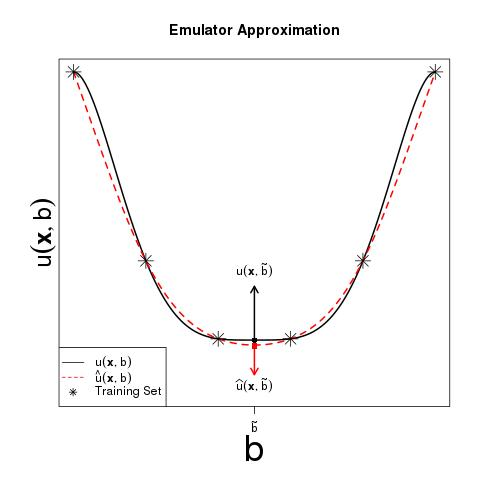
\includegraphics[scale=0.55]{./FigChap3/emulatorApproximation}
\caption{Approximation of a model $u(\x;\cdot)$ by the mean of a Gaussian process trained
with six  different  outputs from the model. The mean of the Gaussian process at a point $\tilde{b}$ is taken
as the value $\widehat{u}(\x;\tilde{b})$ of the emulator.}
\label{figGPCreation}
\end{figure}

 
Let us assume that solving
equation (\ref{eqntoyproblem}) is computationally expensive and repeating the calculation for a big range of 
different values of $b$
is not feasible. One way to get around that is by constructing an emulator $\widehat{u}(\cdot)$ that approximates $u(\cdot)$
and is cheap to compute. 
The way we are going to construct $\widehat{u}(\cdot)$ is as follows: for a fixed $\x\in\mathbb{R}^{2}$ we solve equation 
(\ref{eqntoyproblem}) for   $n$  different values of  $b$. We pick the value of $n$ in a way
that the computational cost of computing (\ref{eqntoyproblem}) $n$ times, does not exceed our
computational and time budget. Then use the data $\{b_{j},u(\x,b_{j})\}_{j=1}^{n}$  as a 
training set to create a Gaussian process, as explained in Chapter 2, Section 2.1.1. Finally
for any value $\tilde{b}$ we use the mean of the Gaussian process at that point as $\widehat{u}(\x,\tilde{b})$.
An sketch from the result for approximating an arbitrary model $u(\x;\cdot)$ with an emulator
$\widehat{u}(\x;\cdot)$ is shown
in Figure \ref{figGPCreation}.


For clarity in the exposition, the table below  summarizes the notation 
we are going to use throughout the rest of the chapter.




%Finally use the emulator
%$\hat{M}(\cdot)$ to predict the output of $M(\cdot)$ for as many different values of $b$ as possible. 
%The value of the emulator at the point $(\x,b)$  is going to be denoted by $\hat{u}(\x;b)$. The following
%table summarizes the notation that is going to be used from now on in this Chapter.

\begin{table}[H]
\centering
\begin{tabular}{|c|c|}
\hline 
Symbol & Meaning \tabularnewline 
\hline 
\hline
\hline 
$\tilde{u}(\x;b)$ & \pbox{7cm}{Value of the physical variable at the point $\x$
with parameter $b$.\\} \tabularnewline 
\hline 
\hline
$u(\x;b)$ & \pbox{7cm}{Numerical solution of equation (\ref{eqntoyproblem})
at $\x$ with parameter $b$.\\} \tabularnewline
\hline
\hline 
$\hat{u}(\x;b)$ & \pbox{7cm}{Value of the interpolation of the emulator $\hat{M}(\cdot)$ at the point $\x$ with parameter
$b$\\}.  \tabularnewline
\hline
\hline 
$P:=\{\x_{1},\ldots,\x_{10}\}$ & \pbox{7cm}{Points where the experimental measurements were taken\\}.  \tabularnewline
\hline
\hline 
$\y:=(\tilde{u}(\x_{1};b),\ldots,\tilde{u}(\x_{10};b))$ & \pbox{7cm}{Values of the experimental measurements for the variable $\tilde{u}$\\}.  \tabularnewline
\hline
\end{tabular}

\caption{Summary of symbols used in Chapter 3.}
\label{tabSymboltable}
\end{table}
Let us return to our original goal:  to estimate the value of $b$ that explains  the experimental data 
$\y$ as best as possible. To create the experimental data $\y$ we 
assume that the true value of $b$ is $0,925$. Then, for this value of $b$,  we solve equation (\ref{eqntoyproblem})
using a finite difference five point  stencil approximation for the Laplacian. 
Next we pick  ten points at random in $\Omega$ and save the value of the numerical 
solution $u$ at those location (see Figure \ref{figsolU}).  Finally we add  noise from
a normal distribution with mean zero and standard deviation $0.01$ to each  of the ten values. 
The resulting numbers  are what we use
as the experimental data $\y=(\tilde{u}(\x_{1};b),\ldots,\tilde{u}(\x_{10};b))$. 
Note that the noise added to the data obtained from the
numerical  solution of equation
(\ref{eqntoyproblem}) plays the role of possible  
errors in the experimental measurements plus inaccuracies of the 
model to describe the true behavior of the physical variable $\tilde{u}$.

\begin{figure}[H]
\centering
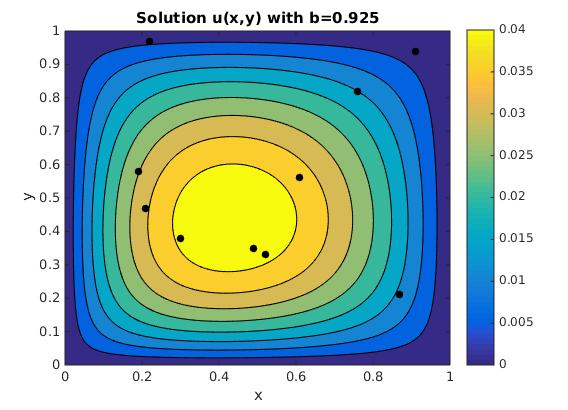
\includegraphics[scale=0.5]{./FigChap3/solu}
\caption{Numerical solution of the system (\ref{eqntoyproblem}) using a five points stencil finite difference
approximation for the Laplacian. The mesh
size used in $x$ and $y$ was $0.01$. The value of the parameter $b$ was set at $0.925$. The black dots
in the plot represent the points used to generate the experimental data 
$\y=(\tilde{u}(\x_{1};b),\ldots,\tilde{u}(\x_{10};b))$}
\label{figsolU}
\end{figure}

With the experimental data $\y$ created, we now proceed to obtain a point estimate value of $b$ that produced that data. 
To that end
we first compute the posterior distribution. We are going to explain step by step how to obtain such distribution.

\section{Computing the Posterior}
To calculate the posterior we use Bayes' rule to get

\begin{equation} \label{eqnpropto}
\post(b|\y)=\frac{\like(\y|b)\prior(b)}{Z(\y)}.
\end{equation}
Note that finding the posterior enables us to obtain   any of point
estimate from equation (\ref{eqnpointestimates}) and the uncertainty associated with that estimate.
To compute $\post(b|\y)$ we need to choose
a prior distribution and the likelihood for $b$. Let us start with the prior. 

\subsection{Choosing the Prior}

For the sake of
the example let us assume that  it is known that
the parameter $b$ cannot be greater than $2$. In this case one way to choose a prior distribution
for $b$ that does not assume any other knowledge than $b\in (0,2]$, is the \textit{uniform distribution}. 
%With this distribution, given a Borel measurable set $A\subset(0,2]$, the probability that $b$ belongs to $A$ is given by
%\begin{equation*}
%\frac{1}{2}\int_{A}dx.
%\end{equation*}
In this case we have 
\begin{equation}\label{eqnpriortoyproblem}
\prior(b)=\frac{1}{2}\textbf{1}_{(0,2]}(b),\qquad\text{for all $b\in\mathbb{R}$},
\end{equation}
where $\textbf{1}_{(0,2]}$ is the indicator function of the set $(0,2]$. The indicator function for a Borel measurable set $C$ is
defined as
\begin{equation*}
\textbf{1}_{C}(y)=\left\{
	\begin{array}{ll}
		1 & \mbox{if }	y\in C\\
		0 & \mbox{if }   y\in C^{c}.
	\end{array}
\right.
\end{equation*}

\subsection{Finding the Likelihood}\label{secFindingLike}
To calculate the likelihood,first we need to know how the set of possible measurements 
$\y=(\tilde{u}(\x_{1};b),\ldots,\tilde{u}(\x_{10};b))$ is related to $b$ when
we let $b$ to vary. Since we don't know the experimental values of the physical variable $\tilde{u}$
for different values of $b$, it is necessary to approximate the relation between $\tilde{u}$ and $b$
by the relation between $u$ and $b$.
To obtain such relation we need to solve
equation (\ref{eqntoyproblem}). By solving  this equation explicitly we can find a functional relation
between $u$ and $b$ for each one of the ten locations depicted in Figure \ref{figsolU}.
It is possible to  solve analytically  equation (\ref{eqntoyproblem}). However
the relation between $u$ and $b$ is  given by an infinite series.  Indeed equation 
(\ref{eqntoyproblem}) is  Poisson's equation with homogeneous boundary conditions. This
equation can be solve using an eigenfunction expansion \cite{logan2014applied}. The
eigenfunctions of the Laplacian in the unit square are given by
\begin{equation*}
\phi_{mn}=\sin(n\pi x)\sin(m\pi y),\qquad\text{for }m,n\in\mathbb{N},\
\end{equation*}
with eigenvalues
\begin{equation*}
\lambda_{mn}=(n\pi)^{2}+(m\pi)^{2}.
\end{equation*}
The eigenfunction expansion  for $u$ in equation (\ref{eqntoyproblem}) is 
\begin{equation*}
u=\sum_{n=1}^{\infty}\sum_{m=1}^{\infty} a_{mn}\phi_{mn}
\end{equation*}
where
\begin{equation}\label{eqnIntegrals}
a_{mn}\lambda_{nm}=-\frac{\int_{\Omega}e^{-b\|x\|^{2}}\phi_{mn}d\x}{\int_{\Omega}\phi_{mn}^{2}d\x}=
-\frac{\langle e^{-b\|x\|^{2}},\phi_{mn}\rangle}{\|\phi_{mn}\|_{L^{2}(\Omega)}^{2}}.
\end{equation}
The symbol $\langle\cdot,\cdot\rangle$ represents the standard inner product in $L^{2}(\Omega)$.


Having a functional relation given
by an infinite series is often not very useful. For example in equation (\ref{eqnIntegrals})
the integral on the numerator does not have a closed form.
Hence we need a different approach to gain insight into the relation between $\y$ and $b$. 
The  approach  we will use is the  same as the one that allowed us to obtain
Figure \ref{figGPCreation}.  First we solve equation (\ref{eqntoyproblem}) for
$n$ different values of $b$. For the sake of the example assume $n=10$. Then 
for each $\x$ in $P=\{\x_{1},\ldots,\x_{10}\}$ we use the
set $\{b_{j},u(\x_{k};b_{j})\}_{j=1}^{10}$ to train a Gaussian process for each $k=1,2,\ldots,10$.
Finally for any $\tilde{b}\in (0,2]$ we use the mean of the Gaussian process at that point as
the value $\widehat{u}(\x_{k};\tilde{b})$. By proceeding in this manner we obtain 
a cheap method to approximate  the behavior   of 
$\y=( \tilde{u}(\x_{1};b),\ldots,\tilde{u}(\x_{10};b))$ when we let 
$b$ to vary.

The next step is to choose  the values of $b$  for which the  PDE (\ref{eqntoyproblem}) is solved in a 
way the uncertainty associated with to the emulator is as small as possible. 
We shall denote the points we choose as $\{b_{1},\dots,b_{10}\}$. To choose the points 
we use a maximin design as explained in Chapter 2 Section \ref{secDesignofExperiments}. In this case
it is straightforward to check that the maximin design is the set of equidistant points
\begin{equation*}
\{b_{1}=0.2,b_{2}=0.4,\ldots,b_{10}=2\}.
\end{equation*}
\newline 
By solving equation (\ref{eqntoyproblem}) for these values of $b$ and for 
each $\x$ in $P$, we know the values in the set $\{u(b_{j},\x_{k})\}_{j,k=1}^{10}$.
%We  use  the set of equidistant  points to train a GP for each of the ten sites in $P$. 
We use this set  to train ten Gaussian Process. With these processes we define the functions 
\begin{equation*}
G_{k}:(0,2]\rightarrow\mathbb{R}\qquad\text{for }k=1,2,\ldots 10.
\end{equation*}
such that  for each $k$ and $b$,  the value of the mean of the $k$-th GP is going to be given by $G_{k}(b)$.
That is, $G_{k}(\cdot)$ is the emulator for $u(\x_{k},\cdot)$. More precisely
\begin{equation*}
G_{k}(b)=\hat{u}(\x_{k};b).
\end{equation*} 

The functions $G_{k}(\cdot)$ are cheap to evaluate and are a good 
approximation of $\tilde{u}(\x_{k},\cdot)$. Now it is possible
to approximate the value of $b$ that explains $\y=(\tilde{u}(\x_{1},b),
\ldots,\tilde{u}(\x_{10},b))$ by trying a big number of different values
of $b$ and then compare with the experimental data, to see what choice
of $b$ gives the smallest discrepancy. To this end, we calculate
the values of $G_{k}(\cdot)$, for $k=1,\ldots,10$ in the set
\begin{equation*}
\{0.01,0.02,\ldots,1.99,2\}.
\end{equation*}

 
In Figure \ref{fignofitted} are plotted  
the emulator at these points,  the true value of $b$, the experimental measurement $\tilde{u}(\x_{k};b)$
and the training data $\{u(\x_{k};b_{j})\}_{j=1}^{10}$ for each of the ten sites.



%
%We are ready to run the emulator $\hat{f}$ for these values of $b$, get a numerical value at
%the 10 points in the domain where the synthetic data were created (black dots in Figure \ref{figsolU})
%and use GPs to fill the missing information. Take into account that this process of `filling the blanks'
%has to be done in all of the 10 measurement points in the domain $\Omega$ of definition of the phyiscal model.
%
%In Figure \ref{fignofitted} we can see the results from running the emulator (black dots) compared
%with the experimental measurement for each of the 10 sites (black line).






We are now ready to make the mathematical connection between $\tilde{u},u$ and $\hat{u}$. Recall
that $u$ is the mathematical approximation of the physical variable $\tilde{u}$ and $\hat{u}$
is an emulator for $u$. Hence if $\hat{u}$ approximates well $u$, we would expect that 
$\hat{u}$ approximates $\tilde{u}$. For any point $\x_{k}\in P$ we do not know exactly
how  $\hat{u}(\x_{k},\cdot)=G_{k}(\cdot)$ differs from $\tilde{u}(\x_{k},\cdot)$.
If we define $y_{k}(b):=\tilde{u}(\x_{k},b)$, then, a possible 
relation
that connects these quantities is given by the following Gaussian additive model \cite{Somersalo}
\begin{equation}\label{eqnreal2interp}
y_{k}(b)=G_{k}(b)+\epsilon_{k},\qquad\text{with } \epsilon_{k}\sim\mathcal{N}(0,\lambda^{2}),
\end{equation}
where $\lambda$ is  a positive number that models how much we believe  the emulator prediction differs from $\tilde{u}$. 
We chose the value $\lambda=5.4\times 10^{-3}$ to get a signal to noise ratio  of 1:10.
By defining the vector  
$\textbf{G}(b)=(\hat{u}(\x_{1};b),\ldots,\hat{u}(\x_{10};b))$ and  the definition of $\y$ 
(see table \ref{tabSymboltable}). Then equation (\ref{eqnreal2interp}) can we written more compactly as
\begin{equation}\label{eqnvector2interp}
\textbf{y}=\textbf{G}(b)+\epsilon,\qquad\text{with }\epsilon\sim\mathcal{N}(0,\lambda^{2} I_{10\times 10}).
\end{equation}


Since the random vector $\epsilon$ has a Gaussian distribution, we can use equation (\ref{eqnvector2interp})
to conclude 
\begin{equation*}
\textbf{y}|b\sim \mathcal{N}(\textbf{G}(b),\lambda^{2} I_{10\times 10}),
\end{equation*}
i.e.
\begin{equation}\label{eqnlikelihoodtoyproblem}
\like(\textbf{y}|b)\propto e^{-\frac{1}{2\lambda^{2}}\|\textbf{G}(b)-\textbf{y}\|_{2}^{2}},
\end{equation}
where the proportionality constant normalizes the distribution on the right hand side to one. 
\newline

\begin{figure}[H]
\centering
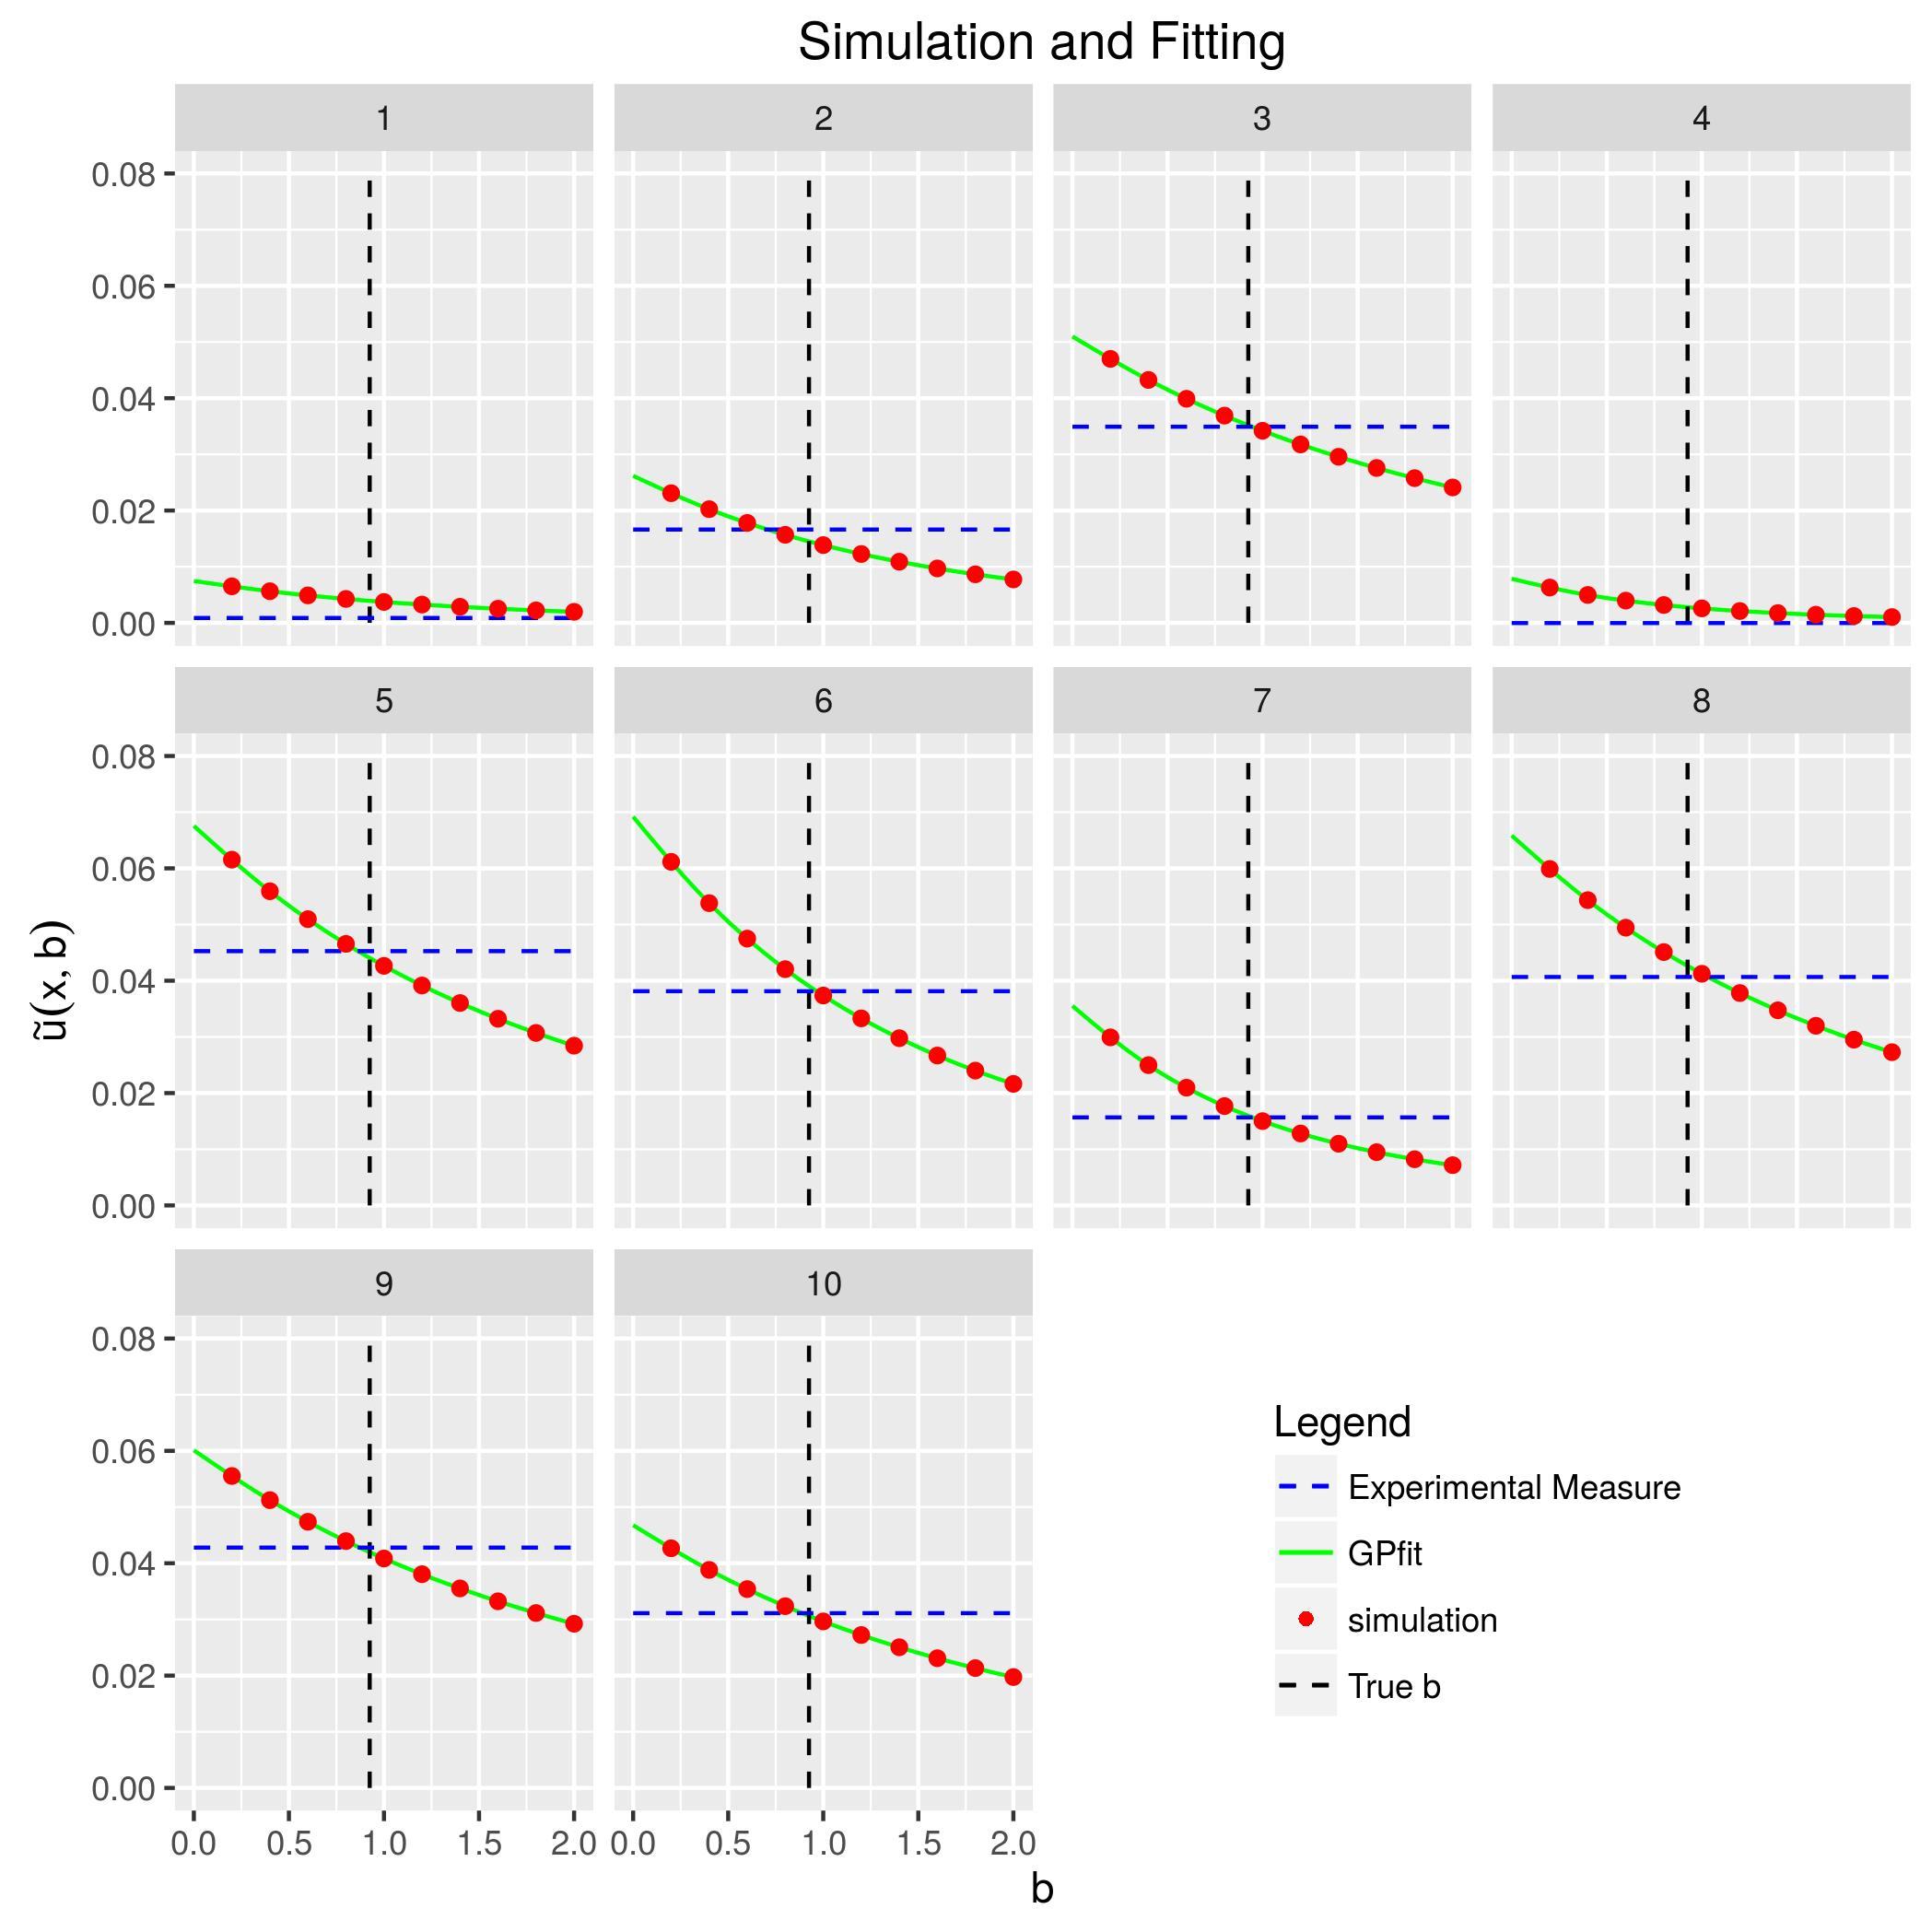
\includegraphics[scale=0.7]{./FigChap3/fitted}
\caption{Training points, GP regression, true value of $b$ and experimental measures for each one of the ten sites labeled
from 1 to 10 in Figure \ref{figsolU}}
\label{fignofitted}
\end{figure}

Now that we have explicit expressions for the prior and likelihood distributions, we
can compute the posterior probability for $b$.
Since
the denominator in Bayes' rule (\ref{eqnpropto}) is independent of $b$, 
we can use equations (\ref{eqnpriortoyproblem}) and (\ref{eqnlikelihoodtoyproblem})  
to write 
\begin{equation}\label{eqnposteriorforb}
\post(b|\y)\propto\like(\y|b)\prior(b)\propto \textbf{1}_{(0,2]}(b)e^{-\frac{1}{2\lambda^{2}}\|\textbf{G}(b)-\textbf{y}\|_{2}^{2}}.
\end{equation}
An interpretation of this result is that before taking experimental measurements  we only knew 
that $b\in (0,2]$. After weighting this prior belief with the data $\y$, our current state of knowledge about the
parameter $b$ is encoded in the posterior distribution. Figure \ref{figlikeprior} shows this updated distribution.
%
%As we can see in Figure \ref{fignofitted}, the emulator sometimes overestimates the value of $b$ and sometimes
%underestimates it, this behaviour is expected. The hope is that this inaccuracies oscilate around the true
%value of $b$.
%
%Since we only have a limited number of prediction of the emulator for different values of $b$ (black points
%in Figure \ref{fignofitted}), we would like to extrapolate/interpolate those results to get
%more data and with that extra data, assess the value of $b$. As explained in Chapter 2, one very useful 
%way to obtain the extra data is through Gaussian processes. Using the language of the previous chapter
%what we want to do is, having the training points $\{(x_{i},f(x_{i})\}_{i=1}^{10}$ we want to predict 
%the value of different test points $x_{i}^{*}$. This prediction is shown as a red line in Figure
%\ref{fignofitted}.  The GP fit allows us to approxiamte as much value as we want, along with the uncertainty
%associated with the prediction. Having this data we can now proceed to use the Bayesian methodology.
%The idea goes as follows. if we denote the GP fit at at point $b$ as  $G(b)$, then we may assume
%an additive noise model for the output $y$ as
%\begin{equation}\label{eqnadditivenoise}
%y=G(b)+\vec{\epsilon}.
%\end{equation}
%$\vec{\epsilon}$ is a random vector distributed as $\vec{\epsilon}\sim\mathscr{N}(0,\sigma I)$. Where $sigma=bla$
%and $I$ is the $10\times 10$ identity matrix.
%In the Bayesian framework we are interest in finding the value of $b$ given the experimental measurements $m$.
%To that end we go back to the begining of this chapter and use equation (\ref{eqnpropto}). To use this equation
%we need to find the likelihood $\like(m|b)$. Under the assumption of the additive noise model in equation
%(\ref{eqnadditivenoise}) we get as in the smashed window example in chapter 2 that
%\begin{equation*}
%m|b\sim\mathscr{N}(G(b),\sigma I),
%\end{equation*}
%more precisely
%\begin{equation*}
%\like(m|b)=\frac{1}{(2\pi\sigma)^{n/2}}\exp\left(-\frac{\|G(b)-m\|_{2}^{2}}{2\sigma^{2}}\right).
%\end{equation*}
%
%
%
%Now we need to choose a prior for $b$. This is a delicate issue and a polemic one in the Statistics community.
%The prior should reflect all of our current knowledge about $b$. However your knowledge about $b$ might be 
%different than my knowledge about $b$, hence your prior for $b$ might look different than mine. For
%the moment  we won't worry about that. Let's assume that our prior for $b$ is given by
%\begin{equation*}
%b\sim U(0,2).
%\end{equation*}
%where $U(a,b)$ is the uniform distribution in $a,b$. Putting all of this into formula (\ref{eqnpropto}) we get
%\begin{equation*}
%\post(b|m)\propto\chi_{[0,2]}\exp\left(-\frac{\|G(b)-m\|_{2}^{2}}{2\sigma^{2}}\right),
%\end{equation*}
%where $\chi_{[a,b]}$ is the indicator function of the set $[a,b]$. This equation can be 
%interpreted as the update in knowledge from to prior to the posterior in the light of the
%experimental data obtained represented by the likelihood. This change from prior to 
%posterior is shown below.
\begin{figure}[H]
\centering
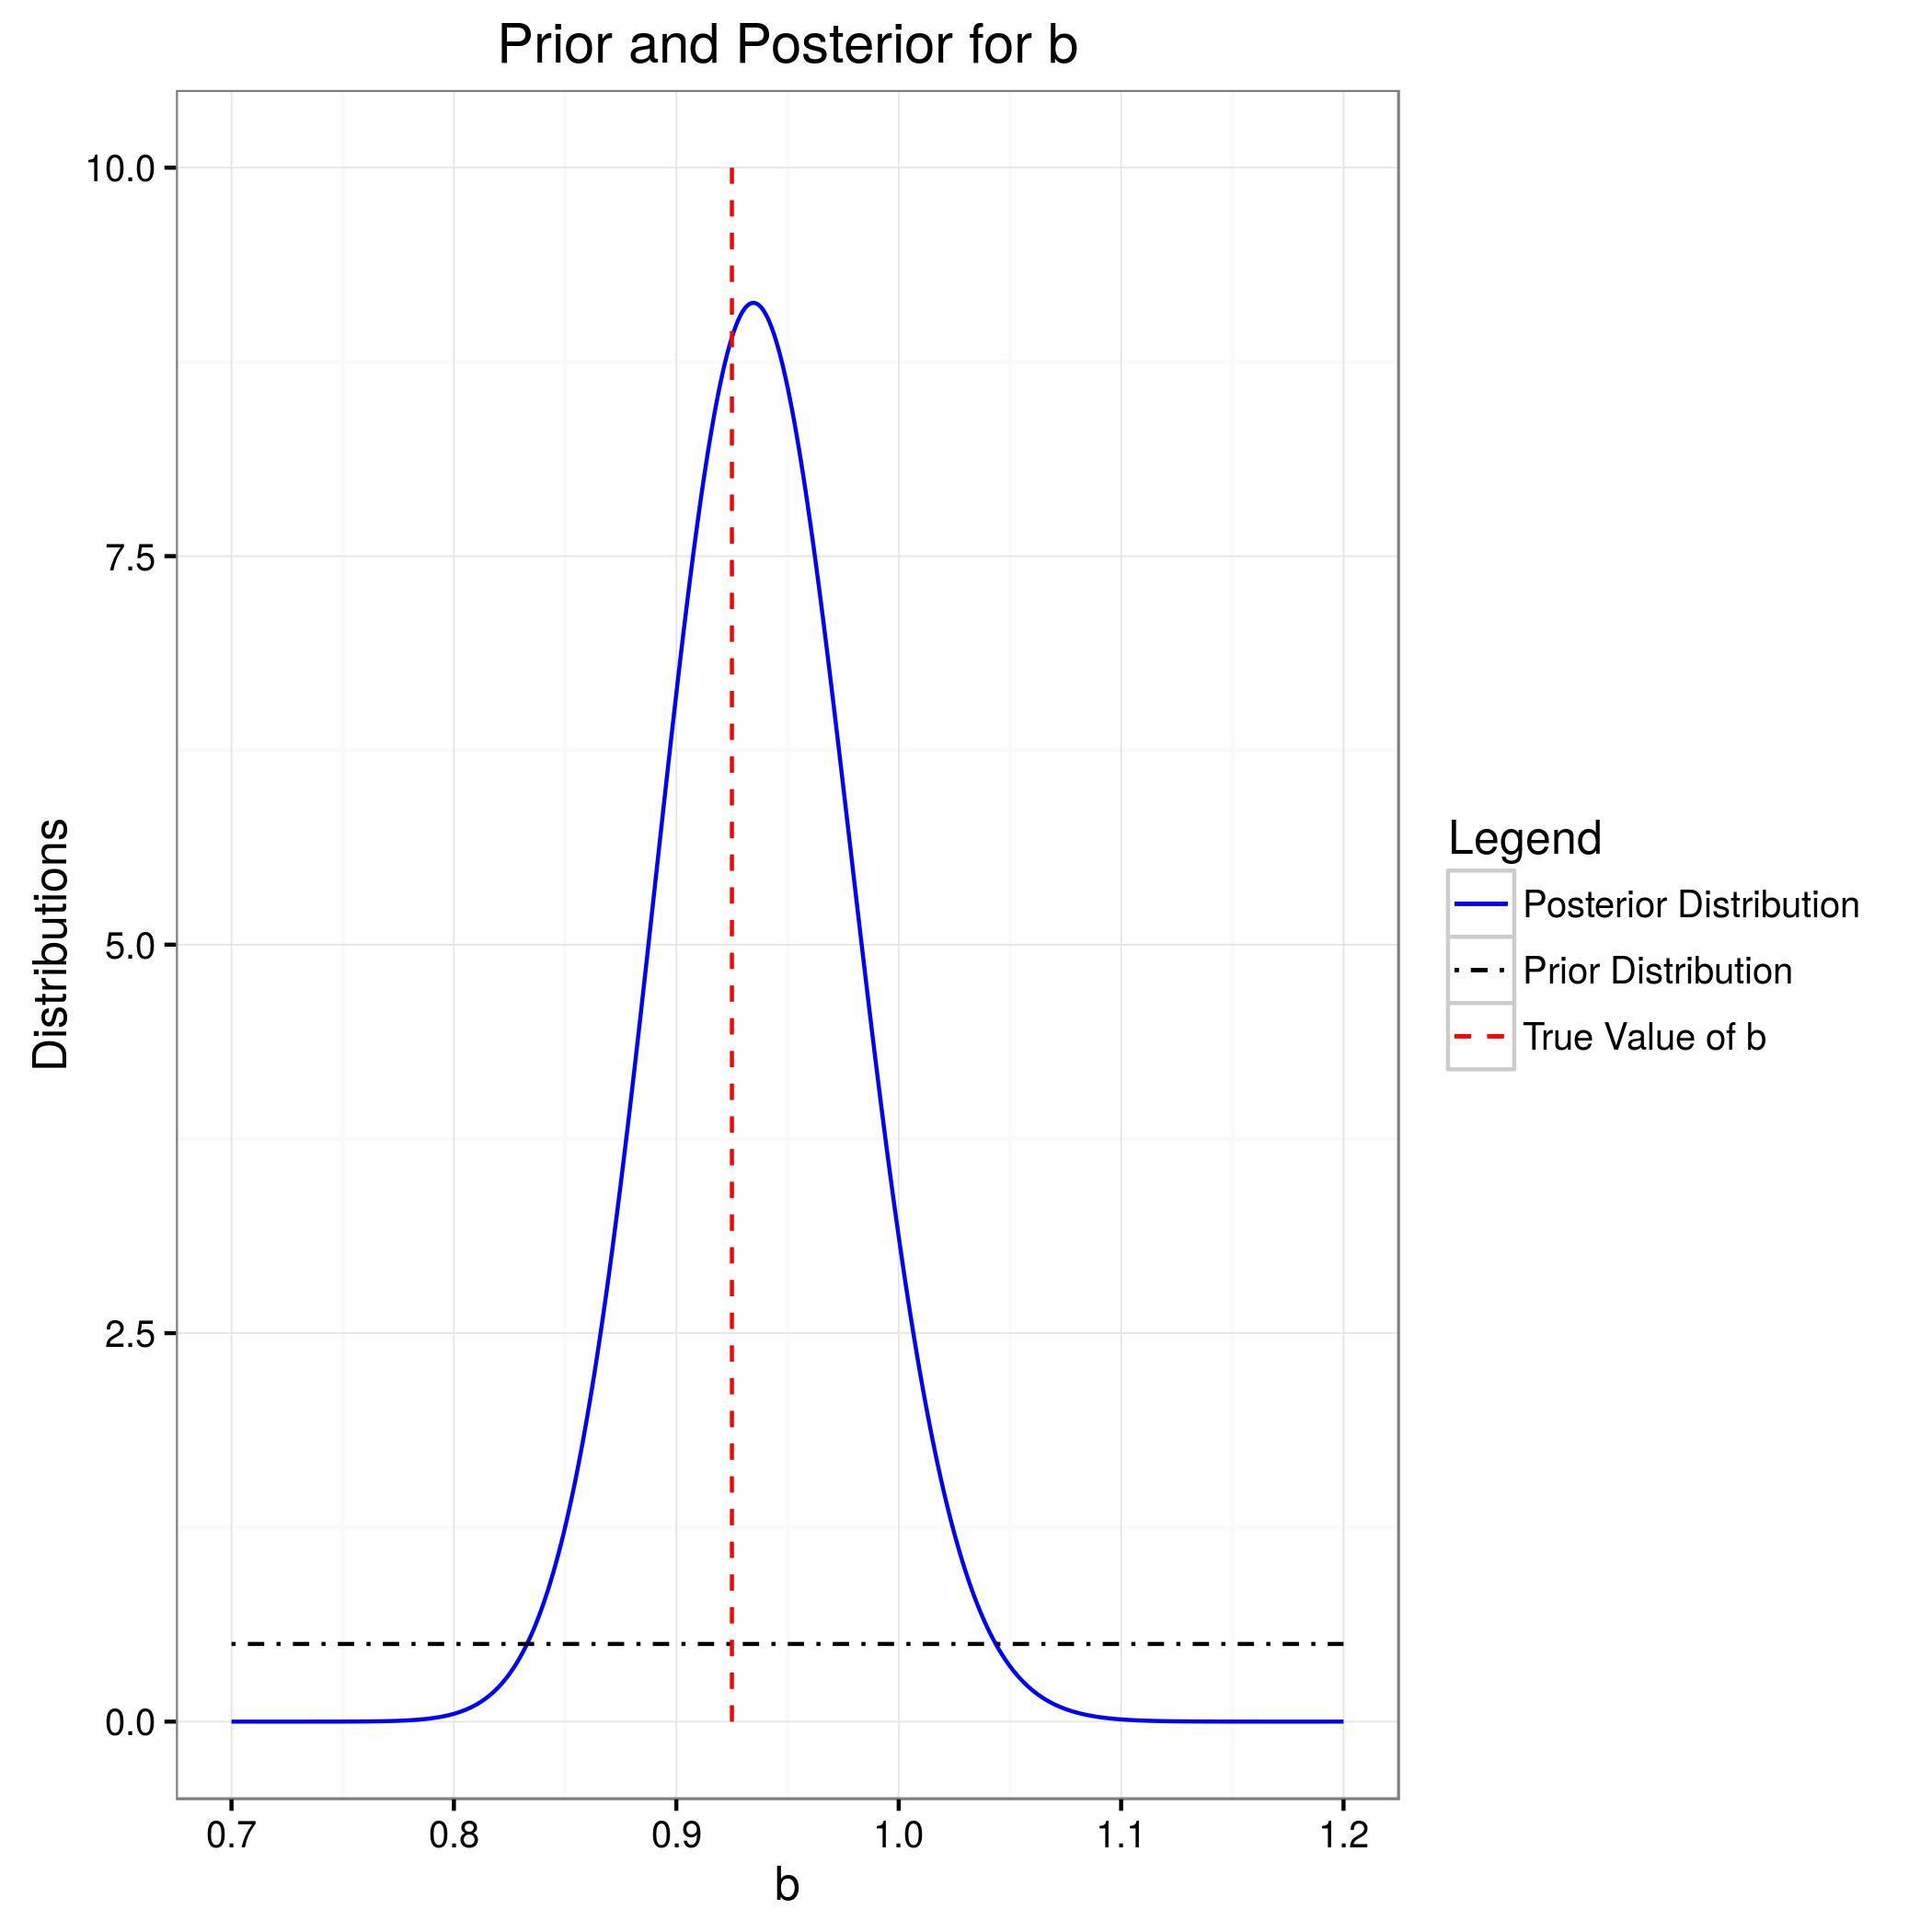
\includegraphics[scale=0.6]{./FigChap3/prior_posterior.jpg}
\caption{Plots of the prior distribution, posterior distribution and true value of the parameter $b$.}
\label{figlikeprior}
\end{figure} 

It is not always possible to visualize a probability density so it is necessary to sample from it
in order to obtain statistics about the parameters of interest.
A family of methods for this purpose
are known as Markov Chain Monte Carlo (MCMC). In this work we 
focus on a particular algorithm known as Metropolis-Hastings  (MH). We now proceed  to explain
how MH works in practice using the posterior for $b$ in equation (\ref{eqnposteriorforb}) as an example. 
\newline
\newline
Consider the posterior density $\post(b|\y)$. The idea is to construct a Markov chain that wanders 
around the support of the posterior
in a way that the chain spends more time in regions with high probability.
One way to achive that is as follows: if we are at a point $q_{1}$ and we want to move to a point $q_{2}$ 
we will accept 
that move with probability one if $\post(q_{1}|\y)\leq\post(q_{2}|\y)$ and with probability 
$\frac{\post(q_{2}|\y)}{\post(q_{1}|\y)}$.  We choose
in what direction to move, randomly, using some probability distribution that is easy to sample from.
For simplicity, In this and the next Chapter we chose the uniform distribution to decide in what  direction to move.
The pseudocode  for the MH algorithm as described above is \cite{Somersalo}

\begin{algorithm}\label{algMH}
\caption{Metropolis-Hastings Algorithm}
\begin{algorithmic}[1]\label{algMH}
\State pick a point $q_{1}$ in the support of the distribution
\For{j=2:N}
\State Draw $u\sim U([0,\alpha])$
\State $q_{j}\leftarrow q_{j-1}+u$
\State $\beta\leftarrow\min(1,\frac{\post(q_{j}|D)}{\post(q_{j-1}|\y)})$
\State Draw $w\sim U([0,1])$
\If{$w<\beta$}
\State $q_{j-1}=q_{j}\qquad$   (Accept the move)
\Else
\State $q_{j-1}=q_{j-1}\qquad$ (Reject the move)
\EndIf
\EndFor
%\\
%\textbf{for} j=2:N
%\item $\qquad$Draw $u\sim U([0,\alpha])$
%\item $$
%\item $\qquad$Compute $\post(q_{j}|D)$
%\item $\qquad$
%\item $\qquad$\\
%\\
%$\qquad\qquad\qquad$\textbf{if} $w<\beta$ 
%\item $\qquad\qquad q_{j-1}=q_{j}$\qquad(Accept move)\\
%\\
%$\qquad\qquad$\textbf{else}
%\item
%	$\qquad\qquad q_{j-1}=q_{j-1}$\\
%\textbf{end}\\
%\textbf{end}
\end{algorithmic}
\end{algorithm}

The rule of thumb for choosing the parameter $\alpha$ in the scheme above is that   the proportion of times we accept
a move 
is about $0.25$ \cite{casella2008monte}. It can be shown that the sequence $q_{1},q_{2},\ldots,q_{N}$
are realizations of a Markov chain that in the limit as $N\rightarrow\infty$ are distributed according to the distribution
$\post(b|\y)$. This convergence result works under mild conditions over the distribution that is being sampled.
For more details about the theory behind MCMC methods we refer the reader to \cite{casella2008monte}. 
Since we do not have the computational power to let $N\rightarrow\infty$. We let the chain run for a large number of steps
until it converges. Then, we throw away the \textit{burn-in} portion of the chain and compute statistics using 
the remaining samples.  The burn-in portion of the chain are the samples obtained before the chain is close 
to converge. A common choice is to discard the first $\frac{N}{2}$ samples.
\newline


Using Algorithm 1, we sample from the posterior distribution $\post(b|\y)$ setting the values $\alpha=0.23$
and $N=10000$. The  burn-in  period is set to be  the first $5000$ samples. An histogram of the last $5000$
is shown below.

%Returning to the problem of sampling the posterior distribution for $b$. We are going to use the Metropolis Hastings algorithm
%using an step size of $\delta=0.23$, $10000$ samples and we chose the first $5000$ to be the burning period. The results 
%of applying the MH algorithm is shown below  
%


\begin{figure}[H]
\centering
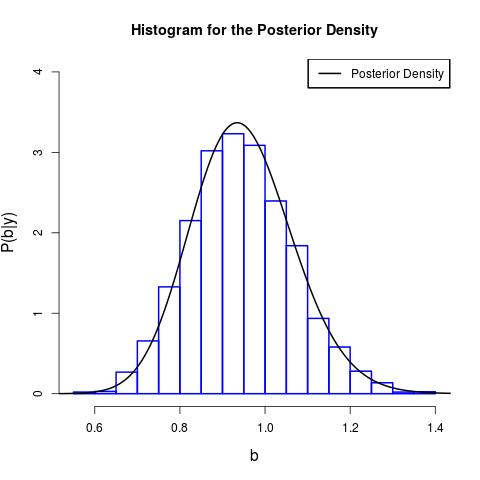
\includegraphics[scale=0.60]{./FigChap3/histogram_mcmc.jpg}
\caption{Histogram obtained for the posterior distribution (\ref{eqnpropto}) 
from $5000$ samples from MH algorithm with step size $\alpha=0.23$. The solid line
is the  graph for the posterior $\post(b|D)$.}
\end{figure}

With the samples obtained we readily obtain useful statistics for $b$. For example, we can estimate
the conditional mean using \cite{casella2008monte}

\begin{equation}\label{eqnbcmMC}
b_{cm}=\int_{(0,2]}b\post(b|D)db\approx\frac{1}{5000}\sum_{j=1}^{5000}b_{j}=0.9247042,
\end{equation}
where the summands $b_{j}$ are the samples obtained after the burn-in period of $5000$ samples. We can 
also estimate the variance of the samples as
\begin{equation*}
\int_{(0,2]}(b-b_{cm})^{2}\post(b|D)db\approx\frac{1}{5000}\sum_{j=1}^{5000}(b_{j}-b_{cm})^{2}=0.01427.
\end{equation*}
With these values we can compute a $95\%$ confidence interval for $b$. In this
case the interval is given by 
\begin{equation*}
[0.9247042-2\sqrt{0.01427},0.92470422+2\sqrt{0.01427}]=[0.68579,1.163618].
\end{equation*}


Let us do a short digression about the idea behind Monte Carlo integration. 
Consider the generic problem of evaluating the $n$-dimensional
integral
\begin{equation}\label{eqnmontecarlo}
\int_{\mathbb{R}^{n}}h(x)\rho(x)dx,
\end{equation}  
where $\rho$ is the Lebesgue density of some probability measure $\p$. This means that calculating (\ref{eqnmontecarlo}) 
is equivalent to calculating the expected value of $h$, i.e.
\begin{equation*}
\mathbb{E}[h]=\int_{\mathbb{R}^{n}}h(x)\rho(x)dx.
\end{equation*}
If we have $X_{1},\ldots,X_{n}$ random variables independent with density $\rho$, then by the strong law of large numbers, the sequence of random
variables
\begin{equation*}
h_{n}=\frac{1}{n}\sum_{k=1}^{n} h(X_{k}),
\end{equation*}
converges to $\mathbb{E}[h]$\cite{dudley2002real}. Furthermore if $\mathbb{E}[h^{2}]<\infty$ we can assess the speed of
convergence and the quality of the approximation $h_{n}$ for $\mathbb{E}[h]$. By the central limit theorem
the sequence of random  variables $h_{n}$
\begin{equation*}
\frac{h_{n}-\mathbb{E}[h]}{\sqrt{\sigma_{n}}}\rightarrow \mathcal{N}(0,1),
\end{equation*}
where 
\begin{equation*}
\sigma_{n}=\frac{1}{n}\sum_{k=1}^{n}(h(X_{k})-h_{n})^{2}.
\end{equation*}
This means that the uncertainty in the approximation $h_{n}$ for $\mathbb{E}[h]$ goes to $0$ as $\mathcal{O}(\frac{1}{\sqrt{n}})$.
Note that the convergence rate is independent of the dimension of the problem. That is the reason why Monte Carlo integration
is used in high dimensional problems, where quadrature methods are prohibitively  expensive to implement. In Chapter 4 we are going to apply 
this method to calculate integrals of real valued functions supported in a seven dimensional space.

The estimate for $b$ in equation (\ref{eqnbcmMC}), depends on the choice of the prior. At this point it is unclear
how choosing a different prior would give a different estimate for $b$.
To close this chapter we discuss  the role that the prior has in inference in the Bayesian Framework.
\section{The Importance of the Prior}
Once again  consider  problem of estimating
the value of the parameter $b$, whose real value is, as before, $0.925$. This time we assume the parameter
$b$ can be any real number (not just $0<b\leq 2$ as before) and the  prior distribution for $b$ to be
\begin{equation*}
b\sim\mathscr{N}(b^{*},\sigma_{b}^{2}),
\end{equation*}
where $b^{*}$ and $\sigma_{b}$ are parameters to be set later.  With this new prior the formula
for the posterior is 
\begin{equation*}
\post(b|\textbf{y})\propto\underbrace{\exp\left(-\frac{\|\textbf{y}-\textbf{G}(b)\|_{2}^{2}}{2\sigma^{2}}\right)}_{\text{Likelihood}}\underbrace{\exp\left(-\frac{(b-b^{*})^{2}}{2\sigma_{b}^{2}}\right)}_{\text{Prior}}.
\end{equation*}
To illustrate the role that the prior has in the inference of the value
of the parameter given the data $\textbf{y}$, suppose that 
\begin{equation*}
b\sim\mathscr{N}(4,2.5).
\end{equation*}
This prior assumes that, with $95\%$ of confidence, the value of
$b$ is in the interval $[1.8,8.2]$. Clearly, there is a mismatch between
the true value of $b$ and the range of values that the prior distribution
assigns high probability. Let us evaluate how the posterior
distribution for $b$ evolves as we consider more and more experimental
data from the measurements of $\tilde{u}$. Figure \ref{figpostevolution} shows
how the posterior evolves when we calculate the likelihood with more 
and more data. The first frame shows the result when only the measurement
$\tilde{u}(\x_{1};b)$ is taken into account. The second frame
when the measurements $\tilde{u}(\x_{1};b),\tilde{u}(\x_{2};b)$ are taken
into account. In each new frame we proceed adding one more measurement 
to calculate the likelihood.

\begin{figure}[H]
\centering
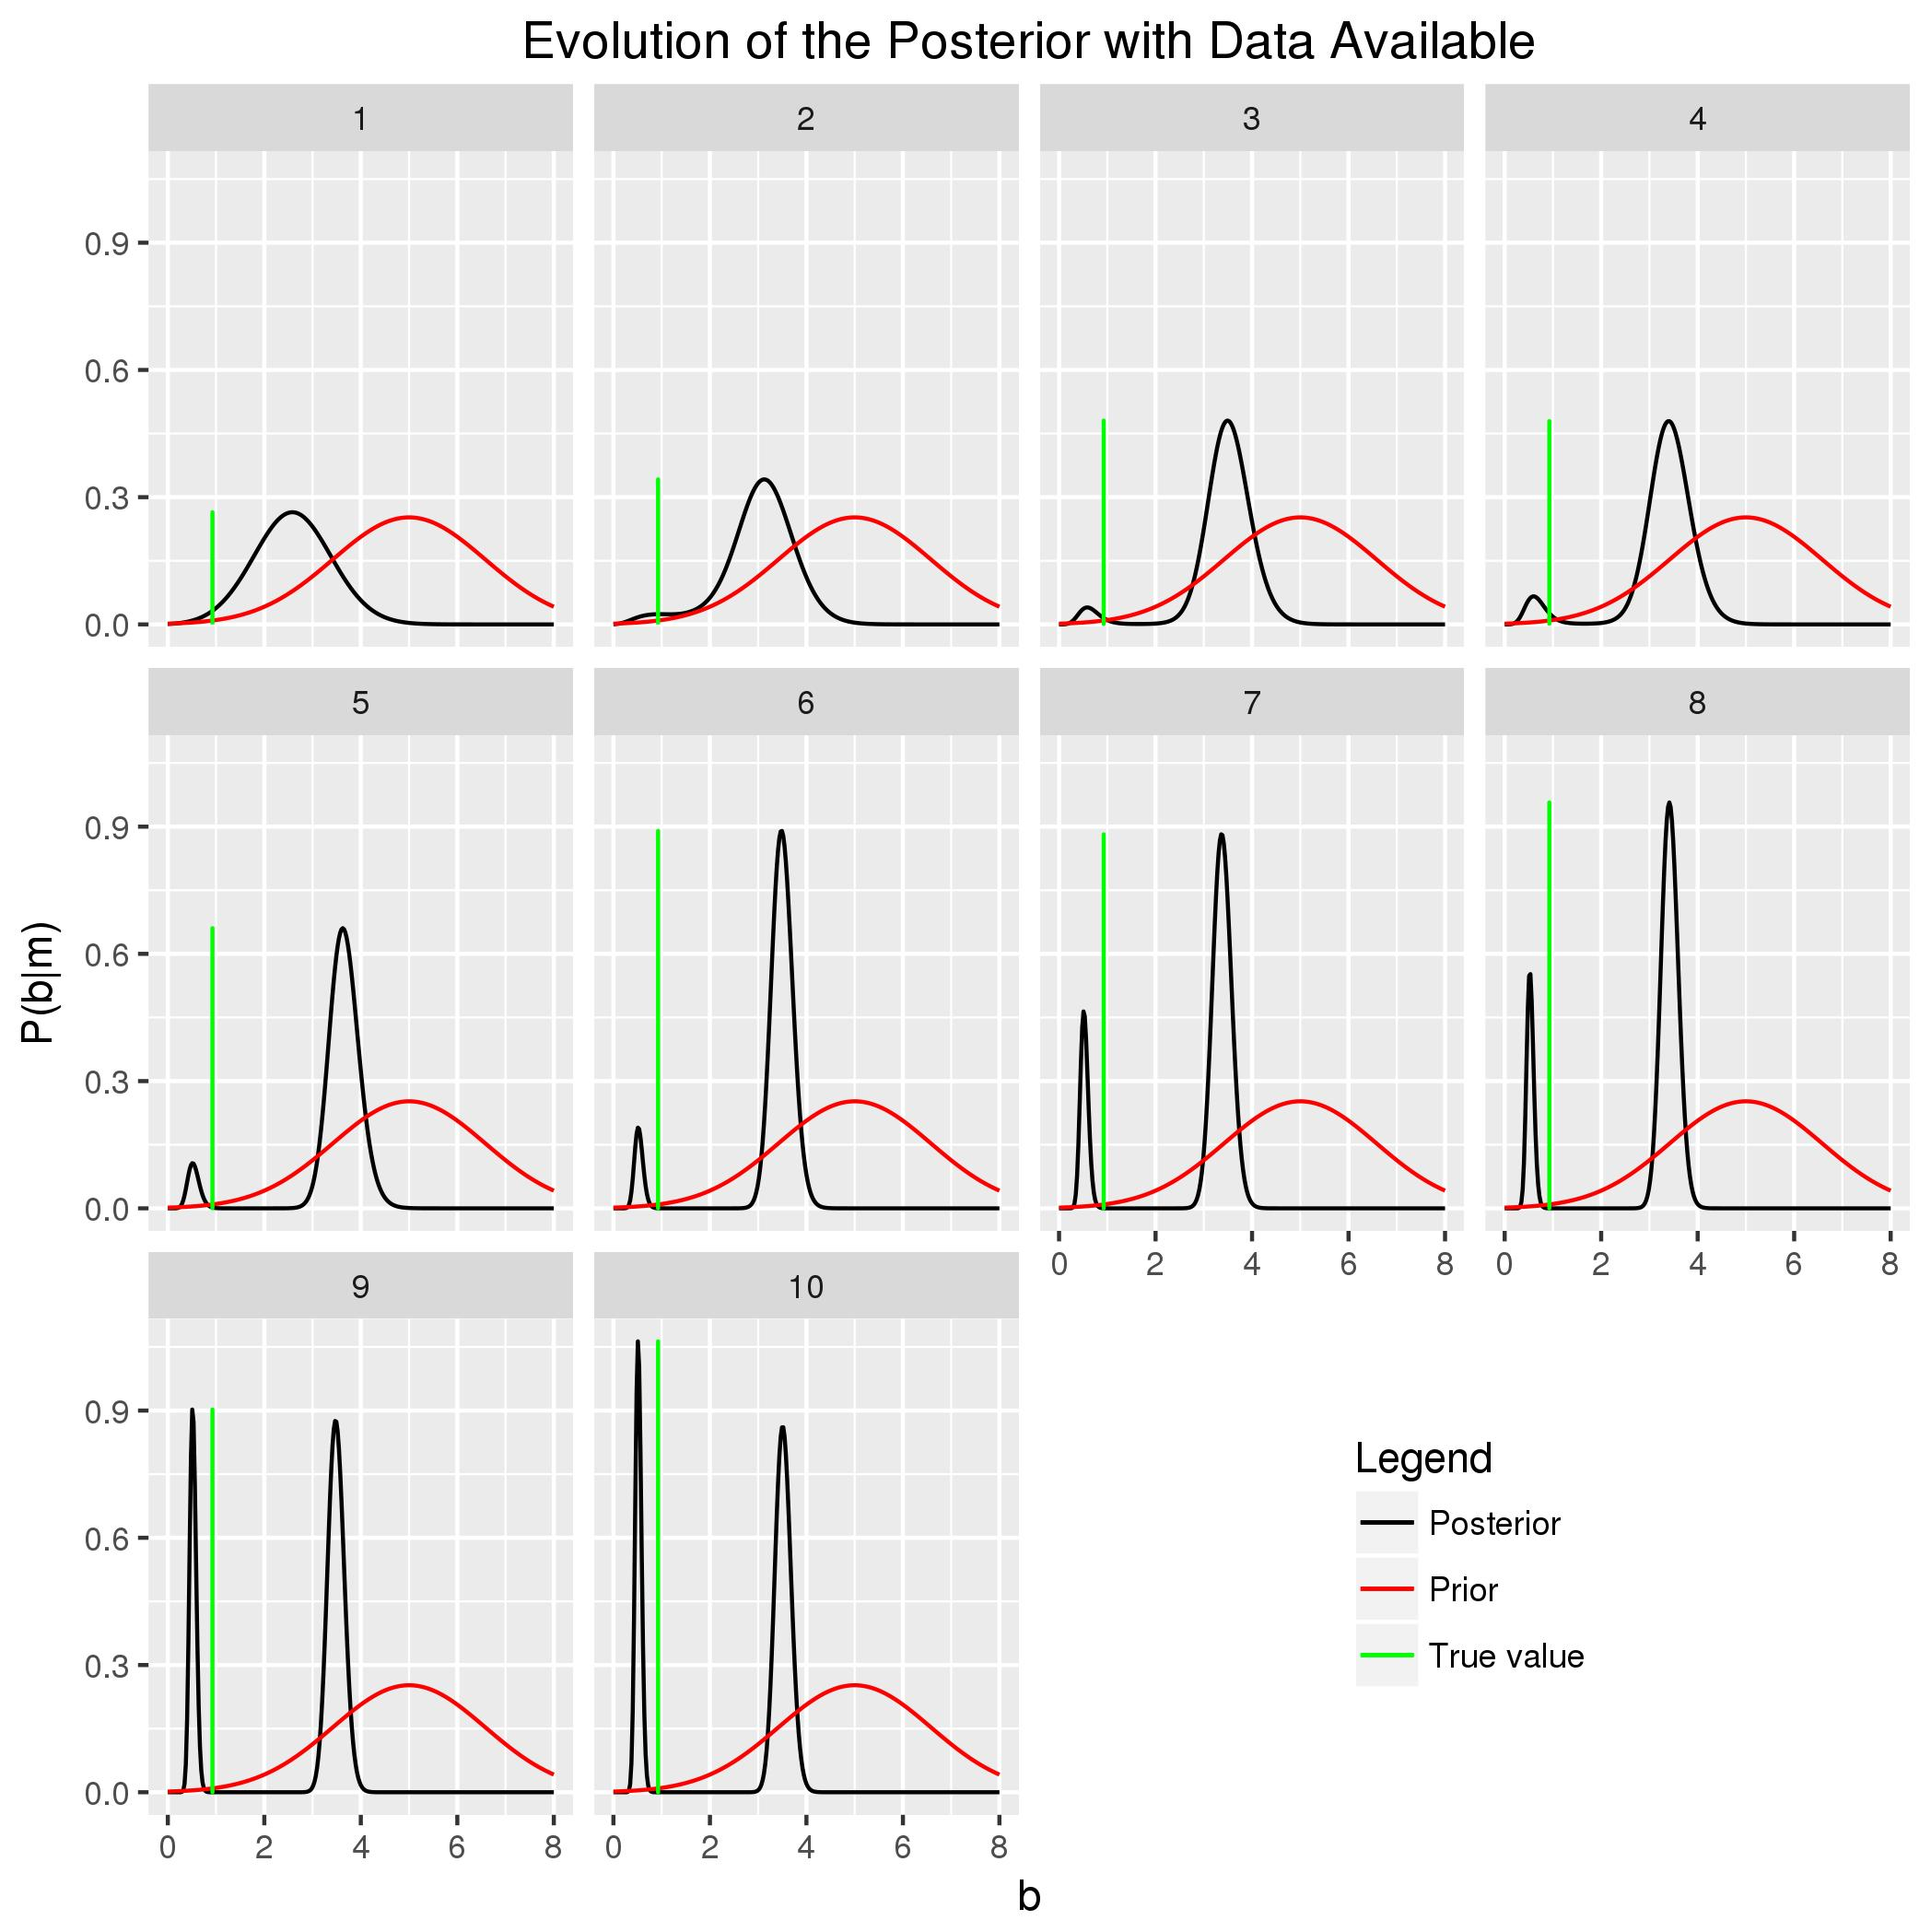
\includegraphics[scale=0.7]{./FigChap3/posterior_evolution}
\caption{Evolution of the posterior distribution when more experimental data is taken into account}
\label{figpostevolution}
\end{figure}

The sequence of plots in Figure \ref{figpostevolution} shows that the experimental data creates a new mode
in the posterior distribution that is close to the true value of $b$. In the end of the sequence where we consider
all 10 experimental measurements, the mode that is close to the true value of $b$ is bigger than the mode originated
by the prior at the point $b=4$. The explanation for this behavior  is that the prior  has a high value near $b=4$, 
but it is close to zero for values around $b=0.925$.
Then, when the experimental data is used, the likelihood distribution has a higher  value for points  close to $b=0.925$
than points close to $b=4$. The more data, the higher the value of the likelihood around $b=0.925$ and closer to zero
away from it. However since
the prior distribution gives negligible probability to values close to the true value of $b$, when all data are used the 
product $\prior(\y|b)\p(b)$ will be non-negligible only in regions close to $b=4$ or $b=0.925$.

The above example is a warning example. If we know how to choose the prior distribution in a way that is meaningful to the
problem, reliable inference could be done even with small amount of data. On the contrary if the prior distribution
is not realistic, inference could not be done or  may not be reliable even with a large amount of data.  
\newpage

%%%%%%%%%%%%%%%%%%%%%%%%%%%%%%%%%%%%%%%%%%%%%Chapter 4 %%%%%%%%%%%%%%%%%%%%%%%%%%%%%%%%%



\chapter{Industrial Case Problem}



As mentioned in the introduction, our interested is to study
the dispersion of zinc from a lead-zinc smelter in Trail, British Columbia, Canada,
operated by Teck Industries Ltd.  The smelter has four smokestacks. From now
on the smokestacks are going to be referred as source. Our goal
is to estimate how much  each source is contributing to the total amount of zinc
that is being released by the smelter.
To this end, we count on experimental
measurements of the zinc deposition at nine different locations and wind velocity data 
of the surrounding area. We also know prior estimates of the zinc release by the smelter.
These estimates where calculated by the engineers that work there.
An aerial photograph of the region  of interest with 
the location of the sources and the measurement devices is shown 
in Figure \ref{figAereal}. The sources are represent by the letters
$Q_{1}$ to $Q_{4}$. The zinc deposition measurement sites are represented
by the letter $R_{1}$ to $R_{9}$. 

To obtain the estimates mentioned in the previous paragraph, we are going
to proceed in the same manner as in estimating the parameter $b$ in equation (\ref{eqntoyproblem})
in Chapter 3. In that Chapter we were given  a mathematical model that approximates
the physics of interest. For this chapter, it is necessary to develop, from scratch,
a mathematical model that approximates the physics behind pollutant dispersion in the
atmosphere. To propose this mathematical model in detail is the topic of the next section.



\begin{figure}[H]
\centering
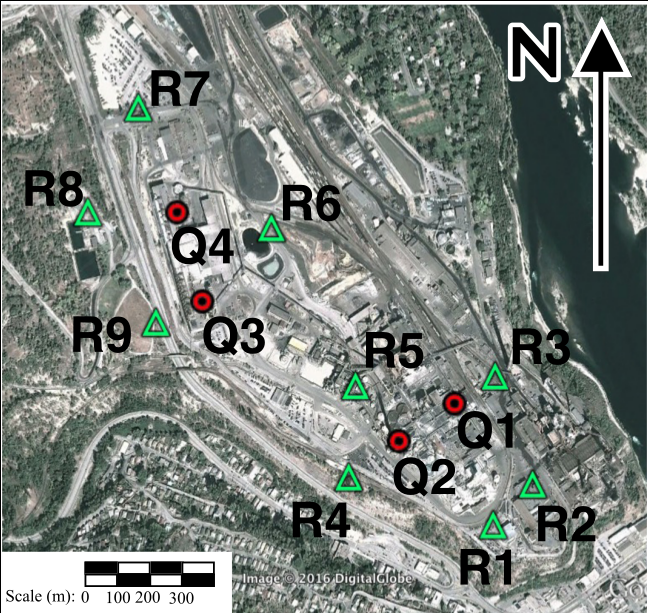
\includegraphics[scale=0.35]{FigChap4/AerealView}
\caption{Aereal photograph of the lead-zinc smelter in Trail, British Columbia, Canada. The points
$Q_{1}$ to $Q_{4}$ represent the sources of zinc. The green triangles $R_{1}$ to $R_{9}$ represent
the location of the measurement devices.}
\label{figAereal}
\end{figure}

%To estimate the contribution of the sources we are going to proceed in the same
%manner as in the previous chapter. First we formulate the mathematical model
%that describes the physics of interest. With the model we proceed to find
%the likelihood. Next we use any given information about the source to choose
%a prior




\section{A Mathematical Model for Pollutant Dispersion}
Our starting point  is the conservation of mass. In particular conservation of mass for
particulate zinc in the atmosphere. Consider a region $\Lambda\subset\mathbb{R}^{3}$ with $m$ units of   mass
of zinc within it. 
Assume
that in the interior of $\Lambda$ there is  a source of  zinc. Furthermore assume that zinc is flowing throughout 
the boundary $\partial\Lambda$ of $\Lambda$  due to a  wind velocity field (see Figure \ref{figControlVolume}).
If $\vv(\x,t)$ represents the wind velocity at a point $\x$ at time $t$, it can be shown that net mass
per unit time, of zinc that is flowing through the boundary is given by the expression
\cite{seinfeld1998atmospheric}
\begin{equation*}
\oint_{\partial\Lambda}c(\x,t)\vv(\x,t)\cdot\hat{\textbf{n}}dA,
\end{equation*}
where  $c(\x,t)$ is the concentration of zinc at a point $\x$
at time $t$.
The units of $c$ are given in units of mass per units of volume. On the other hand
the rate of change total mass $m$ at a time $t$ inside $\Lambda$  can be calculated as
\begin{equation*}
\frac{dm(t)}{dt}=\frac{d}{dt}\int_{\Lambda}c(\x,t)dV.
\end{equation*}

\begin{figure}[H]
\centering
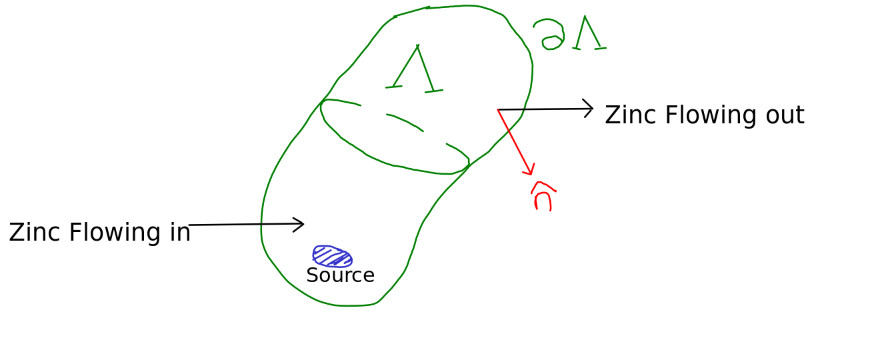
\includegraphics[scale=0.5]{./FigChap4/controlVolume}
\caption{Schematic representation of a volume region in space containing a source of Zinc.}
\label{figControlVolume}
\end{figure}

Finally, the amount of zinc that comes from the source at a time $t$ is given by
\begin{equation*}
\int_{\Lambda}s(\x,t)dV,
\end{equation*}
where $s(\x,t)$ is the source density. Its units are mass per unit volume per unit time.
Conservation of mass states that the total mass inside $\Lambda$ should be conserved. Therefore
for all times the rate of change of the mass inside $m$ should equal all source of variation of it.
Mathematically we can write
\begin{equation*}
\frac{d}{dt}\int_{\Lambda}c(\x,t)dV=-\oint_{\partial\Lambda}c(\x,t)\textbf{v}\cdot\textbf{n}dA+\int_{\Lambda}s(\x,t)dV.
\end{equation*}
Since we picked the orientation of $\partial\Lambda$ with the normal pointing outwards, it is
necessary to put a minus in front of the surface integral for consistency. Assuming
the concentration and the velocity field are continuous functions of time and space, an 
straightforward application of the divergence theorem and Leibniz rule for integral gives
\begin{equation*}
\int_{\Lambda}\left(\frac{\partial c(\x,t)}{\partial t}+\nabla\cdot(c\textbf{v})-s(\x,t)\right)dV=0.
\end{equation*}
Since the region $\Lambda$ was arbitrary, the previous equality holds if and only if
\begin{equation}\label{eqnDeterministic}
\frac{\partial c(\x,t)}{\partial t}+\nabla\cdot(c\textbf{v})=s(\x,t).
\end{equation}
If we apply this equation to estimate the concentration of zinc using real wind data, we 
will find that the prediction for the concentration is not completely accurate. 
The reason is that at small scales, there
are random fluctuations in the wind velocity. To model this we follow \cite{seinfeld1998atmospheric}
and write the wind velocity field as
\begin{equation}\label{eqnNewV}
\vv=\bar{\vv}+\vv',
\end{equation}
where $\bar{\vv}$ is the measured wind velocity and $\vv'$ is a random variable with zero mean.
If we replace $\vv$ in equation (\ref{eqnDeterministic}) with the expression for velocity
in equation (\ref{eqnNewV}) we get
\begin{equation}\label{eqnNewRandom}
\frac{\partial c(\x,t)}{\partial t}+\nabla\cdot(c(\bar{\textbf{v}}+\vv'))=s(\x,t).
\end{equation}
The presence of the random variable $\vv'$ transforms the solution $c$ into a random 
variable as well. In this case we describe $c$ as the contribution of two terms as 
\begin{equation}\label{eqnNewC}
c(\x,t):=\E(c)(\x,t)+c(\x,t)',
\end{equation}
where $c'$ satisfies $\E(c(\x,t)')=0$. The intuition behind this definition is the following: if we repeat a large number of times the experiment
of measuring the concentration at a point $\x$ and at time $t$ under identical initial and boundary condition,  then, we expect the 
measurements to have an underlying average behavior $\E(c)(\x,t)$ plus some  noise $c(\x,t)'$.
Plugging in  equation (\ref{eqnNewC}) into equation (\ref{eqnNewRandom}) we obtain
\begin{equation}\label{eqnInconsistent}
\frac{\partial\E(c)}{\partial t}+\dv(\bar{\vv}\E(c))+\dv(\E(c'\vv'))=s(\x,t).
\end{equation}
This equation includes  the extra variable $\E(c'\vv')$.
In this case we have two unknowns and one equation. 
One way to overcome this issue is given by the so-called mixing-length theory. The
theory uses the constitutive equation
\begin{equation*}
\E(c'\vv')=\textbf{D}\nabla(\E(c)).
\end{equation*}
The term $\textbf{D}$ is  a rank two tensor called the eddy diffusivity tensor. This tensor is assumed 
to be symmetric, hence is always diagonalizable. We may assume that we are working
on the principal axis of $\textbf{D}$ \cite{seinfeld1998atmospheric}, hence 
\begin{equation*}
\textbf{D}=\begin{bmatrix}
D_{xx}& 0 & 0\\
0 & D_{yy} & 0\\
0 & 0 & D_{zz}
\end{bmatrix}.
\end{equation*}
Under the mixing-length theory, equation (\ref{eqnInconsistent}) reads as
\begin{equation}\label{eqnfirstDifferentialForm}
\frac{\partial\E(c)}{\partial t}+\dv(\bar{\vv}\E(c)+\textbf{D}\nabla\E(c))=s(\x,t).
\end{equation}
The variable $\E(c)$ is a deterministic function of space and time. So to make
notation lighter,  we set $C(\x,t):=\E(c)$. Note that $C$ has the same units
as $c$. We interpret $C(\x,t)$ as the expected concentration we would measure
at the point $\x$ at time $t$.

For the source density we assume point-wise sources. If there are $n$ sources 
 at the points $\x_{1},\x_{2},\ldots,\x_{n}$, located inside the domain of definition 
of equation (\ref{eqnfirstDifferentialForm}),
then we assume a source density of the form
\begin{equation}\label{eqnSourceDensity}
s(\x,t)=\sum_{j=1}^{n}q_{j}(t)\delta(\x-\x_{j}).
\end{equation}
Here $q_{j}$ is referred as the  strength of the $j$-th source and has units of mass per unit time. 
The function $\delta(\cdot)$ is the Dirac delta function. For our model we have $n=4$ sources 
(see Figure \ref{figAereal}). Taking into account the observations made in the 
previous paragraph, we finally state the mathematical model for zinc disperssion as
\begin{equation}\label{eqnDifussivityFinalForm}
\frac{\partial C(\x,t)}{\partial t}+\dv(\bar{\vv}C(\x,t)+\textbf{D}\nabla C(\x,t))=\sum_{j=1}^{4}q_{j}(t)\delta(\x-\x_{j}).
\end{equation}



Due to the presence of the diffusivity tensor, it is necessary to make assumptions about
the behavior of the diagonal elements of $\textbf{D}$. Also the measurements of the wind velocity 
are given by one 2-axis anemometer. This means we count with just one wind velocity measurement at
 one point in space. This means it is also necessary to make assumption about
the wind velocity distribution. 


\subsection{Assumptions on the Diffusivity Tensor}
Following \cite{monin1954basic},  the vertical diffusivity coefficient $D_{zz}$ is approximated by
\begin{equation}\label{eqnEddyVertical}
D_{zz}=\frac{\kappa v_{*} z}{\phi(z/L)},
\end{equation}

Where $\kappa$ is the \textit{Von-Karman} constant whose value in practice is set as $0.4$. The denominator
is defined as the piece-wise continuous function
\begin{equation*}
\phi\left(\frac{z}{L}\right)=\left\{
			\begin{array}{ll}				
				1+4.7\frac{z}{L} &\mbox{for }\frac{z}{L}>0 \\
				1 &\mbox{for }\frac{z}{L}=0\\
				(1-15\frac{z}{L})^{-\frac{1}{2}}&\mbox{for }\frac{z}{L}<0
			\end{array}.
		\right.
\end{equation*}
Here $L$ is referred as the \textit{Monin-Obukhov length}. Finally the parameter $v_{*}$ is known as 
the \textit{friction velocity}.  This parameter is calculated as 

\begin{equation*}
v_{*}(t)=\frac{\kappa v_{r}(t)}{\ln(\frac{z_{r}}{z_{0}})},
\end{equation*}
where $v_{r}(t)$ is a reference velocity at a reference height $h_{r}$. The variable $z_{0}$ 
is called the \textit{roughness length}. 

For the elements $D_{xx}$ and $D_{yy}$, we assume $D_{xx}=D_{yy}$ and independence of height 
\cite{monin1954basic}. A common used equation
to approximate these variables is given by
\begin{equation*}
D_{xx}=D_{yy}\approx \frac{v_{*}z_{i}^{\frac{3}{4}}(-\kappa L)^{-\frac{1}{3}}}{10}.
\end{equation*}
The variable $z_{i}$ is known as the \textit{mixing layer height}.

\subsection{Assumptions on the Wind Velocity Distribution}
In practice, the wind velocity measurements are done using anemometers that  
measure a two dimensional projection of the   velocity vector field.
Therefore
it is necessary to make assumptions on the three dimensional and global behavior of this vector field.
Following \cite{hosseini2016airborne}, we assume a velocity vector field of the form 
\begin{equation}\label{eqn2Dvel}
\vv=(v_{x}(z,t),v_{y}(z,t),v_{set}).
\end{equation}
Observe it is assumed  the wind velocity field is independent of $x$ and $y$.
In equation \ref{eqn2Dvel}, $v_{set}$ is a constant given by  the settling velocity of the zinc particles. By Stoke's law,
this velocity is given by
\begin{equation*}
v_{set}=\frac{\rho g d^{2}}{18\mu},
\end{equation*}
where $\rho$ is the particle density, $g$ the acceleration of gravity,  $d$ its diameter, and
$\mu$ is the air viscosity. For the $x,y$ components of $\vv$ we assume a power law relation of the form
\begin{equation}\label{eqnPowerLaw}
\|(v_{x}(z,t),v_{y}(z,t))\|_{2}=v_{r}(t)\left(\frac{z}{z_{r}}\right)^{p},
\end{equation}
where $v_{r}(t)$  is the wind speed at a reference height $z_{r}$. The exponent $p$ depends on 
factors such as the surface roughness and atmosphere stability. For more details in the power
law model for the wind velocity the reader is referred to \cite{seinfeld1998atmospheric}.
\newline
Observe that the  diffusivity coefficient in equation (\ref{eqnEddyVertical}) vanishes
at the ground level. This is inconsistent with the boundary condition in equation (\ref{eqnRobinBoundary}).
Hence, we assume the diffusivity coefficient to be non-zero below a \textit{cutting height} $z_{cut}$.


Assuming an specific form for the wind velocity and the  
diffusivity tensor, introduces new parameters whose values need to be set. In our model
there are five parameters we need to assign a value before we can use equation (\ref{eqnDifussivityFinalForm}).
These parameters are
\begin{itemize}
\item $p$: the fitting parameter for the wind velocity power law.
\item $z_{0}$: roughness length
\item $z_{i}$: mixing layer height.
\item $L$: Monin-Obukhov length.
\item $z_{cut}$ cutting height.
\end{itemize}
In practice we set a value for these parameters from a given interval of numbers
that empirically has shown to work \cite{seinfeld1998atmospheric,hosseini2016airborne}.
The caveat with this approach is that there is no good reason to choose one value
over a different one. In this work we will  use the Bayesian framework
to decide the values of these parameters and the sources as well.

To completely specify the model for the zinc pollutant dispersion, it is necessary to specify the domain of interest, 
the   boundary and initial  conditions in equation (\ref{eqnDifussivityFinalForm}).
The spatial domain of interest is given by
\begin{equation*}
\Pi:=\{(x,y,z)\in\mathbb{R}^{3}|z\geq 0\}.
\end{equation*}
Following \cite{hosseini2016airborne}, the boundary conditions are given by the far-field condition
\begin{equation*}
C(\x,t)\rightarrow 0\qquad\text{as   }\|x\|\rightarrow\infty,
\end{equation*}
and the Robin boundary condition
\begin{equation}\label{eqnRobinBoundary}
\left.\left(v_{set}C+D_{zz}\frac{\partial C}{\partial z}\right)\right\rvert_{z=0}=\left.v_{dep}C\right\rvert_{z=0}.
\end{equation} 
\newline

To estimate the parameters $p$, $z_{0}$, $z_{i}$, $L$, $z_{cut}$  and  the four sources sources, we count on  experimental measurements 
of the zinc deposition at the sites 
$R_{1},\ldots,R_{9}$ (see Figure \ref{figAereal}) over one month period. The mathematical model described so far,
approximates the physics of the 
concentration, not the deposition. Thus is necessary to make the connection between the solution $C$ of equation (\ref{eqnDifussivityFinalForm})
and the deposition of zinc at $z=0$. If $v_{set}$ is the settling velocity of zinc particles,
it is not hard to see that the deposition per unit area at a point $(x,y,0)\in\Pi$ during the interval of time $(0,T]$ is given by
\begin{equation}\label{eqnw}
w(x,y,T)=\int_{0}^{T}C(x,y,0,t)v_{set}dt.
\end{equation}

Since the nine measurements $R_{1},\ldots,R_{9}$ were obtained by the placement of identical dust-fall jar collectors with non-zero, but small 
cross-sectional area,
we can readily approximate the total deposition during the interval $(0,T]$ at the $i$-th site as
\begin{equation*}
W(x_{i},y_{i},T)=\int_{dust-fall}w(x,y,T)dxdy\approx w(x_{i},y_{i},T)\Delta A,
\end{equation*}
where $\Delta A$ is the cross-sectional area of the dust-fall jar. To make notation lighter we define
\begin{equation}\label{eqnW}
M_{i}=W(x_{i},y_{i},T)\qquad\text{ for }i=1,\ldots,9.
\end{equation}
The scalar $M_{i}$ is the zinc deposition at the site $R_{i}$. From now on we assume $T$ to 
be one month. 

From equations (\ref{eqnw}) and (\ref{eqnW}),
we infer that the map that takes concentration into deposition is linear. Also from equation
(\ref{eqnDifussivityFinalForm}) it is straightforward to check that the concentration $C$
is related to the source $s(\x,t)$ by a linear partial differential operator. Since composition
of linear maps is linear, we conclude that the map that takes sources to deposition is linear.
Since we have four different sources, which we denote by $q_{1},q_{2},q_{3},q_{4}$, we may write
\begin{equation}\label{eqnLinComb}
M_{i}=\sum_{j=1}^{4}a_{ij}(p,z_{0},z_{i},L,z_{cut})q_{j}\qquad\text{for }i=1,\ldots, 9.
\end{equation}
The coefficients $a_{ij}$ capture the dependence of the deposition with respect to the
parameters $p,z_{0},z_{i},L,z_{cut}$, which in general is non-linear. If 
we define the vectors
\begin{eqnarray*}
\y& = &\begin{bmatrix}
M_{1}&\ldots & M_{9}
\end{bmatrix}^{T}, \\
\textbf{q}&=&\begin{bmatrix}
q{1}&q_{2}&q_{2}&q_{4}
\end{bmatrix}^{T},
\end{eqnarray*}
we can write equation (\ref{eqnLinComb}) more compactly as
\begin{equation}\label{eqnLinRel}
\y=A(p,z_{0},z_{i},L,z_{cut})\textbf{q}.
\end{equation}
Here $A$ is a $9\times 4$ matrix whose coefficients are $a_{ij}(p,z_{0},z_{i},L,z_{cut})$.
\newline

Equation (\ref{eqnLinRel}) models the relation between deposition and all
parameters involved in equation (\ref{eqnDifussivityFinalForm}). However we do not 
know an expression for the 36 coefficients $a_{ij}$ as a function of
$(p,z_{0},z_{i},L,z_{cut})$. To find such expression it is necessary
to solve equation (\ref{eqnDifussivityFinalForm}). There is no known closed
form of this equation, hence a numerical approximation is necessary. If we
had unlimited computational or time budget we could solve equation 
(\ref{eqnDifussivityFinalForm}) for as many different configurations
of the parameters $(p,z_{0},z_{i},L,z_{cut})$ as we want and use these
results to approximate the coefficients $a_{ij}$. Clearly this 
is not feasible. A more realistic approach is to solve equation (\ref{eqnDifussivityFinalForm})
for a number of different configurations of $(p,z_{0},z_{i},L,z_{cut})$ that does not
exceed our computational and time budget. Then use Gaussian processes
to interpolate at the configurations we did not solve. Before we proceed to
use Gaussian processes for the interpolation let us see if is possible
to reduce the dimensionality of the parameter space. 
To this end, we do  sensitivity analysis, as explained in Chapter 2, Section \ref{subsecSensitivity}.


\section{Sensitivity Analysis}
Our starting point is to consider the set of  maps $\{\varphi_{x,y}\}_{x,y\in\mathbb{R}^{2}}$. The input
for each map is a point $(p,z_{0},z_{i},L,z_{cut})$ in the parameter space
and the output is the deposition value at the point $(x,y)$. The domain
of each map is the set of allowed values for the parameters. The
range of allowed values for the set of parameters is shown in Table  \ref{tabRanges}\cite{seinfeld1998atmospheric}.


\begin{table}[H]
\centering
\begin{tabular}{|c|c|c|}
\hline 
Parameter (units) & Symbol & Range\tabularnewline
\hline 
\hline 
Velocity exponent  & $p$ & ${[}0.1,0.4{]}$\tabularnewline
\hline 
Roughness length (m) & $z_{0}$ & ${[}10^{-3} ,2{]}$\tabularnewline
\hline 
Height of mixing layer (m) & $z_{i}$ & ${[}10^{2},3\times 10^{3}{]}$\tabularnewline
\hline 
Monin-Obukhov length (m) & $L$ & ${[}-500,-1{]}$\tabularnewline
\hline 
Cut-off length (m) & $z_{cut}$ & ${[}1,5{]}$\tabularnewline
\hline 
\end{tabular}
\caption{Parameters under study and their accepted ranges}
\label{tabRanges}
\end{table}
We perform a sensitivity analysis as explained in Chapter 2, Section \ref{subsecSensitivity},
on the set of maps $\{\varphi_{x_{i},y_{i}}\}_{i=1}^{9}$ ,
where $(x_{i},y_{i})$ represent the location $R_{i}$ in Figure \ref{figAereal}.
To make computations
simpler we map bijectively the set of ranges of the parameters into the five-dimensional
unit hypercube $[0,1]^{5}$. Thus, without lost of generality we may assume the deposition maps are of the form 
\begin{equation*}
\varphi_{x_{i},y_{i}}:[0,1]^{5}\subset\mathbb{R}^{5}\rightarrow\mathbb{R}\qquad\text{for }i=1,2,\ldots,9.
\end{equation*} 

Recall from  Chapter 2, Section \ref{subsecSensitivity}, that in order to estimate
Sobol indices is necessary to perform numerical integrations over the integrands $\{\varphi_{x_{i},y_{i}}\}_{i=1}^{9}$.
These integrals are five-dimensional, hence a quadrature method is not feasible. It is
necessary to use Monte Carlo integration. In order to implement it, is necessary
to know the output of $\{\varphi_{x_{i},y_{i}}\}_{i=1}^{9}$ at any point in their domain. In general we do not
know the output of the function of interest beyond a very limited number of points. 
To extrapolate any function from the set $\{\varphi_{x_{i},y_{i}}\}_{i=1}^{9}$
at  points in its domain where we do not know the output, we use an emulator using Gaussian processes as
explained in Chapter 2, Section \ref{secGPs}.

Implementing the routines to  emulate  and estimate
 Sobol indices is a time consuming task. In order to optimize our time budget, we used
the R packages DiceKriging and Sensitivity \cite{DiceKriging,sensitivity} for the 
emulator and to  estimate the total
effect Sobol index for each of the maps  $\{\varphi_{x_{i},y_{i}}\}_{i=1}^{9}$.  
The DiceKriging package allows us to use five different kernels for the emulation.
In order to consider the influence in using different kernels for the estimation  the Sobol
indices, we calculate the indices five times, one for each different kernel. 
%The results obtined for the sensitivity analysis
%using each of the five different kernels are shown in the box plots in Figure \ref{figSensitivityPlot}.


\begin{figure}[H]
\centering
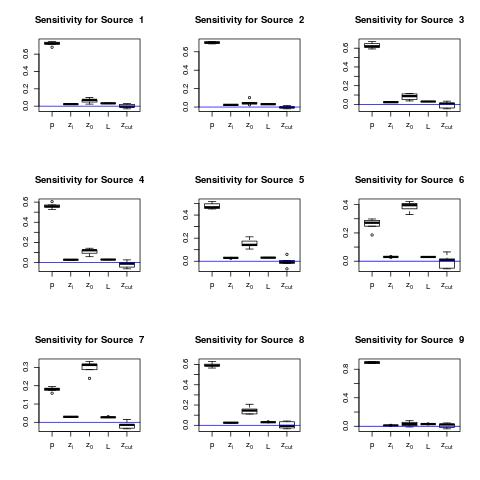
\includegraphics[scale=0.75]{./FigChap4/sensitivityPlot}
\caption{Boxplots containing the result  for the total effect Sobol index performed on each of the nine sensors.
The dashed line represents the value of zero.}
\label{figSensitivityPlot}
\end{figure}
Figure $\ref{figSensitivityPlot}$ shows that two of the five variables do not account for the variance 
in the deposition, namely, $z_{i}$ and $z_{cut}$. Therefore we can reduce the dimensionality of the parameter
space from five to three. In this case we can write equation (\ref{eqnLinRel}) as 
\begin{equation*}
\y=A(p,L,z_{0})\textbf{q}.
\end{equation*}  
From now on we use the convention that the parameters $z_{i}$ and $z_{cut}$ 
are  fixed at the values 100 and 2 respectively (see \cite{hosseini2016airborne}).  
\newline

In order to obtain a closed expression for the matrix $A$ it is necessary to solve 
equation (\ref{eqnDifussivityFinalForm}) along with its boundary condition. There is no known close
form to this equation, hence is necessary to use numerical methods to solve it. Then,
use these results to obtain information about $A$. Solving equation (\ref{eqnDifussivityFinalForm})
is a computationally intensive task. Is not feasible to solve it for a wide range
of different values of $(p,L,z_{0})$. Instead, to 
learn about $A$ we choose an small number of different values of the parameters $(p,L,z_{0})$, and
for the rest of the points we  will use an emulator.



\section{Building an  Emulator for $A(p,L,z_{0})$}

To solve numerically
equation (\ref{eqnDifussivityFinalForm}), we used a finite volume code. The details
of the implementation are given in \cite{hosseini2016airborne}. Running the 
volume code on an $30\times 30\times 30$ grid takes about 30 minutes. Hence the 
necessity to use Gaussian process regression to create an emulator
as explained in Chapter 2, Section \ref{secFindingLike}.

To construct the emulator we need a training set. For that end we create an space filling design for 
the parameter space $(p,L,z_{0})$, as explained
in Chapter 2, Section \ref{secDesignofExperiments}. In  particular
we will use a maximin design. 
Finding a maximin design
is an optimization problem, that is analytically  challenging to solve, hence is
necessary to use numerical approximations. For the optimization  we used 
the particle swarm algorithm. The reader interested in this algorithm
is referred to \cite{arora2015optimization}.  

Considering our time and computational budget, we  chose to 
do the experimental design with $n=64$ points. The maximin
design obtained by using a particle swarm for the 
optimization is shown in Figure \ref{figParticleSwarm}.

With the experimental design completed, the next step is to run the finite volume code 
on each of the different 64 configurations of parameters. We repeat this step four
times. The first time we run the 64 simulations by fixing the first source $q_{1}$ to 1
and the other three sources to zero. The second time we fix the second source $q_{2}$ to 1
and the other three sources to zero. For the third and fourth step we  fix the 
third and fourth source to one respectively, and the rest of the sources to zero. The reason
for this implementation is that we need to connect the output of the finite
volume code, which is the deposition vector $\y$ at the nine sites $R_{1},R_{2},\ldots,R_{9}$
with the components of the matrix $A(p,L,z_{0})$. Recall that the relation between these two quantities 
is given by equation (\ref{eqnLinRel}), explicitly 
\begin{equation}\label{eqnReminder}
\y=A(p,L,z_{0})\underbrace{\begin{bmatrix}
q_{1}\\q_{2}\\q_{3}\\q_{4}
\end{bmatrix}}_{\q},
\end{equation}

For example if we run the finite volume code with the parameters set at the values
$p^{*},L^{*},z_{0}^{*}$ with the $i$-th source set to one and the other 
three to zero, obtaining the output
\begin{equation*}
\y^{*}=\begin{bmatrix}
y_{1}^{*}\\
\vdots\\
y_{9}^{*}
\end{bmatrix}.
\end{equation*}
Then from equation (\ref{eqnReminder}) it is easy to see that 
the following equality holds
\begin{equation*}
\begin{bmatrix}
y_{1}^{*}\\
\vdots\\
y_{9}^{*}
\end{bmatrix}=\begin{bmatrix}
a_{1i}(p^{*},L^{*},z_{0}^{*})\\
\vdots\\
a_{9i}(p^{*},L^{*},z_{0}^{*})
\end{bmatrix}
\end{equation*}

where the RHS is the $i$-th column of $A$. This result shows why
it is necessary to run four times each of the 64 simulations to 
obtain the training set for the emulator of $A$.
The emulator for $A$ will be represented by $\widehat{A}$. The
construction of $\widehat{A}$ is obtained by 
using Gaussian processes as explained in Chapter 2, Section \ref{secGPs}, and
exemplified in Chapter 3 Section \ref{secFindingLike}. By construction,
at the points in the maximin design in Figure \ref{figParticleSwarm}, $A$
and $\widehat{A}$ coincide. To account for the discrepancies outside this
set of points
we assume an additive Gaussian noise model between deposition, parameters
and sources, that is (cf. Chapter 3, Section \ref{secFindingLike})
\begin{equation}\label{eqnChp4Additive}
\y=\widehat{A}(p,L,z_{0})\q+\epsilon,
\end{equation} 
with $\epsilon\sim\mathcal{N}(0,\lambda I_{9\times 9})$. The value of 
the parameter $\lambda$ is going to be set later in the chapter. 
In equation (\ref{eqnChp4Additive})
the vector $\y$ could represent either the output of the finite volume 
code at the dustfall jars positions or the experimental deposition measures. 
This interpretation of $\y$ implies  that the random variable $\epsilon$, also
accounts for the discrepancy between simulation 
of equation (\ref{eqnDifussivityFinalForm}), the physics and 
experimental measurement errors.
\begin{figure}[H]
\centering
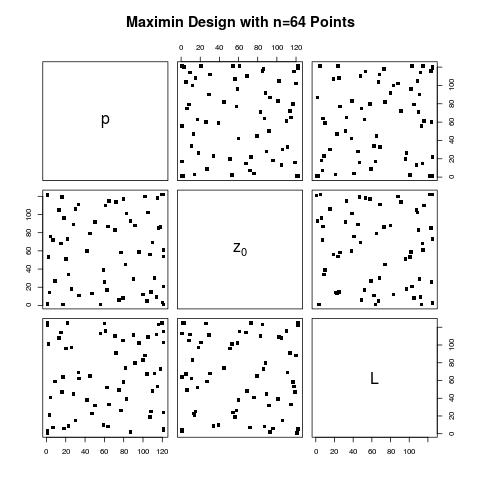
\includegraphics[scale=0.6]{./FigChap4/experimentalDesign64}
\caption{Maximin design with 64 points in the parameter space $(p,L,z_{0})$.}
\label{figParticleSwarm}
\end{figure}


After constructing the emulator, we are now in position to apply
the Bayesian framework to estimate the values for the parameters and the sources. 
This is going to be done in the next section.

\section{Bayesian Framework for the Inverse Problem}

Recall that in the Bayesian framework, to solve an inverse problem
is equivalent to find the posterior distribution of the parameters
of interest. In our case we want to find the posterior
of the parameters $\pars$ and sources $\q$ given
the experimental data $\y$. By Bayes' rule the posterior
distribution is given by
\begin{equation}\label{eqnBayesChp4}
\post(p,z_{0},L,\q|\y)=\frac{\like(\y|p,z_{0},L,\q)\prior(p,z_{0},L,\q)}{Z(\y)}.
\end{equation}
Given the Gaussian additive noise model in equation (\ref{eqnChp4Additive}), 
the likelihood can be calculated as
\begin{equation*}
\y|\pars,\q\sim\mathcal{N}(\widehat{A}\q,\lambda I).
\end{equation*}
or explicitly
\begin{equation}\label{eqnFinalLike}
\like(\y|\pars,\q)=\frac{1}{(2\pi\lambda^{2})^{\frac{9}{2}}}\exp\left(-\frac{1}{2\lambda^{2}}\|\widehat{A}q-\y\|^{2}\right).
\end{equation}




The constant of proportionality is given by
\begin{equation}\label{eqnPropConst}
Z(\y)=\int\like(\y|p,z_{0},L,\q)\prior(p,z_{0},L,\q)dpdz_{0}dLd\q.
\end{equation}
To find it, is necessary to choose a prior distribution. We now
turn our attention into choosing a prior that captures the better the information
we have about the problem.



\subsection{Choosing a Prior}
The values of the  parameters $p,z_{0}.L$ depend on the environmental conditions of the region
where the lead-zinc smelter is, whereas
the values of the sources $q_{1},q_{2},q_{3},q_{4}$ do not. Thus, it is reasonable
to assume that the possible values between these two sets of variables are independent
of each other. This can be captured by the assumption
\begin{equation*} 
\prior(\pars,\q)=\prior(\pars)\prior(\q).
\end{equation*}
By writing the prior distribution as the product of two distributions, we 
simplify the problem by working with two different subsets of variables.
Let us first work with the prior for the parameters $p,z_{0}.L$. In \cite{seinfeld1998atmospheric}
it is propose a function relation of the form
\begin{equation*}
L=a+b\ln(z_{0}),
\end{equation*}
where $a$ and $b$ are constants. This relation is empiric and its validity is yet to be
confirmed. Instead we assume that $z_{0}$ and $L$ are independent. Finally
 there is no known connection between the parameter $p$ and the other two
parameters. Thus we assume all three parameters are independent of each other.
This assumption is  modeled by 
\begin{equation*}
\prior(p,z_{0},L)=\prior(p)\prior(z_{0})\prior(L).
\end{equation*}
As mentioned in Chapter 1, there is no strong reason to pick a value over the other 
for these parameters.
Since there is no preference, we assume an uniform
distribution for each parameter. The allowed range for each parameter is given
in Table (\ref{tabRanges}). Explicitly we have the  distribution
density for each parameter as
\begin{eqnarray}\label{eqnPriorparam}
\prior(p)=\frac{1}{0.3}\textbf{1}_{[0.1,0.4]}\nonumber\\
\prior(z_{0})=\frac{1}{2-10^{-3}}\textbf{1}_{[10^{-3},2]},\\
\prior(L)=\frac{1}{499}\textbf{1}_{[-500,-1]}\nonumber.
\end{eqnarray}
Choosing the prior for the sources $q_{1},q_{2},q_{3},q_{4}$ requires more
analysis since we are not completely ignorant about their possible values. 
Let us summarize our knowledge about these variables.
\begin{enumerate}
\item Each source is unrelated to the other three.
\item $q_{i}>0$ and $q_{i}<\infty$ for $i=1,2,3,4$.
\item According to the engineers working at the smelter, the estimated
output for the sources are
\begin{table}[H]
\centering
\begin{tabular}{|c|c|}
\hline 
Source & Estimated Emission Rate {[}ton/yr{]}\tabularnewline
\hline 
\hline 
$q_{1}$ & 35\tabularnewline
\hline 
$q_{2}$ & 80\tabularnewline
\hline 
$q_{3}$ & 5\tabularnewline
\hline 
$q_{4}$ & 5\tabularnewline
\hline 
\end{tabular}
\caption{Estimated parameters for the four sources.}
\label{tabSources}
\end{table}
\item The engineers estimates are reliable.
\end{enumerate}
Mathematically the first condition can be written as
\begin{equation*}
\prior(q_{1},q_{2},q_{3},q_{4})=\prior(q_{1})\prior(q_{2})\prior(q_{3})\prior(q_{4}).
\end{equation*}
The second condition requires that the probability density for each source has to 
be supported in the set $[0,\infty)$. The third and fourth conditions can be interpreted
as follows: the mode of the prior  for each sources has to be at the
engineers estimated value and $99\%$ of the mass should be contained between 0 and 3
times that value. A probability distribution that 
satisfies the above conditions is the gamma distribution. The gamma distribution
is a parametric distribution. It will be 
denoted by $\mathscr{G}(\alpha,\beta)$. The Lebesgue density
for the gamma distribution is given by
\begin{equation*}
f(x|\alpha,\beta)=\frac{\beta^{\alpha}}{\Gamma(\alpha)}x^{\alpha-1}e^{-\beta x}\textbf{1}_{[0,\infty)},
\end{equation*}
where $\alpha$ and $\beta$ are constants. We are going to assume that each source has 
a  gamma distribution. In this case we write
\begin{equation*}
q_{i}\sim \mathscr{G}(\alpha_{i},\beta_{i})\text{ for }{i=1,2,3,4},
\end{equation*}
or equivalently
\begin{equation}\label{eqnPriorq}
\prior(q_{i})=\frac{\beta_{i}^{\alpha_{i}}}{\Gamma(\alpha_{i})}q_{i}^{\alpha_{i}-1}e^{-\beta_{i} q_{i}}\textbf{1}_{[0,\infty)}.
\end{equation}
We choose the values of $\alpha_{i}$ and $\beta_{i}$  in terms of
the engineer estimate $q_{eng,i}$ for the $i$-th source.
More precisely we choose the values of $\alpha_{i}$ and $\beta_{i}$ 
as the solution of the 
following system of equations
\begin{eqnarray*}
\frac{\alpha_{i}-1}{\beta_{i}}=q_{eng,i}, \\
qgamma(0.99,\alpha_{i},\beta_{i})=3q_{eng,i}.
\end{eqnarray*}
Here $qgamma$ is the quantile function for the gamma distribution. By choosing the values
of the parameters for the gamma distribution in this manner, we satisfy
\begin{equation*}
\max_{q\in [0,\infty)}f(q|\alpha_{i},\beta_{i})=q_{eng,i}\qquad\text{for }i=1,2,3,4.
\end{equation*}
and $99\%$ of the mass of the density is concentrated between 0 and 3 times the
engineers estimate. 
Combining the results from equations (\ref{eqnPriorparam}) and (\ref{eqnPriorq})
we conclude that the prior distribution  satisfies
\begin{equation}\label{eqnPriorFinal}
\prior(p,z_{0},L,\q)\propto \textbf{1}_{[0.1,0.4]}\textbf{1}_{[10^{-3},2]}\textbf{1}_{[-500,-1]}\prod_{i=1}^{4}q_{i}^{\alpha_{i}-1}e^{-\beta_{i} q_{i}}\textbf{1}_{[0,\infty)}.
\end{equation}
With the prior and the likelihood, we finally obtain the expression for the posterior by combining equations (\ref{eqnFinalLike}),(\ref{eqnPropConst}) and (\ref{eqnPriorFinal})
into Bayes' rule in equation (\ref{eqnBayesChp4}). Explicitly,  the posterior $\post(\pars,\q|\y)$ is proportional to
\begin{equation*}
\exp\left(-\frac{1}{2\lambda^{2}}\|\widehat{A}\q-\y\|^{2}-\sum_{i=1}^{4}\beta_{i}q_{i}\right)\prod_{j=1}^{4}q_{i}^{\alpha_{i}-1}\textbf{1}_{[0.1,0.4]\times[10^{-3},2]\times[-500,-1]}.
\end{equation*}


The indicator function represents the ranges of the allowed  values of the parameters in Table (\ref{tabRanges}). 
These values are widely accepted in the literature, however there is not
a technically sounded reason of why these ranges are acceptable.  We will expand the possible values for  these parameters
in order to test the validity of the values in Table (\ref{tabRanges}). The new set of ranges we picked are shown
in Table \ref{tabNewRanges}.


\begin{table}[H]
\centering
\begin{tabular}{|c|c|c|}
\hline 
Parameter (units) & Symbol & Range\tabularnewline
\hline 
\hline 
Velocity exponent  & $p$ & ${[}0,0.6{]}$\tabularnewline
\hline 
Roughness length (m) & $z_{0}$ & ${[}0 ,3{]}$\tabularnewline
\hline 
Monin-Obukhov length (m) & $L$ & ${[}-600,0{]}$\tabularnewline
\hline 
\end{tabular}
\caption{Parameters under study and their new allowed ranges.}
\label{tabNewRanges}
\end{table}
Using these new ranges for the parameters the posterior $\post(\pars,\q|\y)$ is now proportional to

\begin{equation}\label{eqnPosteriorFinal}
\exp\left(-\frac{1}{2\lambda^{2}}\|\widehat{A}\q-\y\|^{2}-\sum_{i=1}^{4}\beta_{i}q_{i}\right)\prod_{j=1}^{4}q_{i}^{\alpha_{i}-1}\textbf{1}_{[0,0.6]\times[0,3]\times[-600,0]}.
\end{equation}
This equation is the solution for the inverse problem. However the formula for the posterior is not of much use. It is
necessary to extract the information contained in it. In order to extract such information we can
obtain point estimates of the parameters and the uncertainty associated to those estimates. 
Finding these estimates is the topic of the next section.



\section{Inferring the Parameters and the sources}

To find  point estimates such as those  in equation (\ref{eqnpointestimates}) and its uncertainty associated,  is necessary to perform  high
dimensional integrals that are not analytically tractable. Thus we resort to use numerical integration techniques. In 
particular   we will use use 
the Metropolis-Hastings(MH) algorithm (see Chapter 3, Algorithm 1) to sample from the posterior and then
use Monte Carlo integration to obtain the quantities of interest. In order to use MH, the posterior
in equation (\ref{eqnPosteriorFinal}), has to be fully specified. Up to this point we have not
set the value of $\lambda$ in the likelihood distribution in equation (\ref{eqnFinalLike}). 
Fixing a value for $\lambda$ is relevant for the model. To understand why this is so, consider
the cases when $\lambda$ is very small and $\lambda$ is very large. In the former case the exponential  term in the likelihood
\begin{equation*}
\exp\left(-\frac{1}{2\lambda^{2}}\|\widehat{A}\q-\y\|^{2}\right),
\end{equation*}
becomes negligible unless $\|\widehat{A}\q-\y\|$ is of the order of $\lambda$. The interpretation
is that we are giving all the credibility to the model and the data. In this case,
the posterior behaves like the likelihood.
In the case when $\lambda$ is large the exponential flattens out. In this scenario
the likelihood is not giving any weight to different combination of the parameters $\pars$ and $\q$,
thus we are giving all the credibility to the prior distribution.
In this case the posterior behaves like the prior. Thus, it is necessary to pick a value of 
$\lambda$ that weights the importance of the likelihood in the right way. By the ``right" way
we mean, a value of $\lambda$ that weights the data, the atmospheric model simulation output and
the prior information equally. To achieve this we propose the value of $\lambda$ that
 minimizes the functional
\begin{equation*}
J(\lambda)=\frac{1}{2}\E_{\post}\left[\|\widehat{A}(p,L,z_{0})\q-\y\|_{2}+\|\q-\q_{est}\|_{2}\right],
\end{equation*}
where $\q_{est}=[35,80,5,5]^{T}\frac{Ton}{yr}$. Explicitly,
\begin{equation}\label{eqnFunctional2Optimize}
J(\lambda)=\frac{1}{2}\int\left(\|\widehat{A}(p,L,z_{0})\q-\y)\|_{2}+\|\q-\q_{est}\|_{2}\right)\post(\pars,\q|\y)dpdLdz_{0}d\q.
\end{equation}
Observe that dependence of $J$ with $\lambda$ comes in the posterior distribution, since different values of $\lambda$
implies we are taking expectation with respect to different probability densities. The motivation
to define $J$ as above is the following: consider
the expression
\begin{equation}\label{eqnPreFunctional}
(1-\delta)\|\widehat{A}(p,L,z_{0})\q-\y)\|_{2}+\delta\|\q-\q_{est}\|_{2},\qquad\text{for }\delta\in [0,1].
\end{equation}
In this case, depending on the value of $\delta$, we are giving different weights to model's credibility,
and the prior information about $\q$. There is no reason to believe the model is more powerful than
the engineers' source strength estimation or vice-versa,  hence by choosing $\delta=\frac{1}{2}$
we weight both terms equally. Also we want to make the term (\ref{eqnPreFunctional}) as small
as possible, regardless of the value of $\pars$ and $\q$, and using the information
contained in the experimental data $\y$. Taking the expectation of \eqref{eqnPreFunctional}
accomplishes that. 

\begin{figure}
\centering
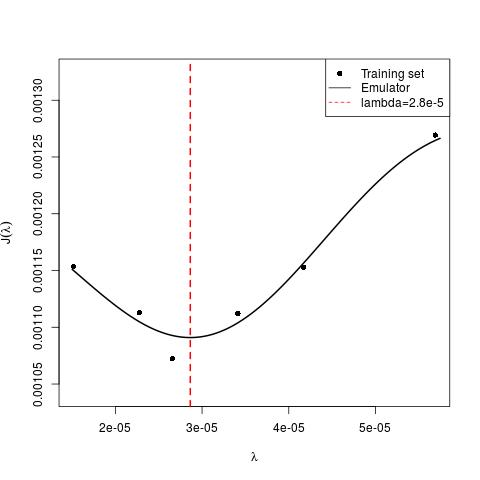
\includegraphics[scale=0.5]{./FigChap4/lambdaEmul}
\caption{bla}
\label{figLambdaEmul}
\end{figure}

Estimating $J(\lambda)$ is expensive, since  it is necessary to evaluate a seven-dimensional
integral. Thus, to approximate a minimizer for $\lambda$  we will use an emulator for $J$ using Gaussian processes. 
To create the training set, we evaluate
$J$ for four different values of $\lambda$ using Markov Chain Monte Carlo integration.
The results of the emulation are shown in Figure \ref{figLambdaEmul}. The minimum for 
$J(\lambda)$ is attain approximately at $\lambda=2.80008\times 10^{-5}$. This
is the value we are going to pick for $\lambda$ to sample from the
posterior distribution in equation \eqref{eqnPosteriorFinal} and use the samples
to obtain point estimates for $\pars$ and $\q$. We mention that if more
accuracy is need in finding the minimizer it is possible to use Gaussian processes
for optimization, we refer the reader to \cite{osborne2009gaussian} for details in this topic.


For the MH implementation we adapt Algorithm 1 in Chapter 3, in a way
that the sampling of $u$ (line 3 in the Algorithm) is done adaptively as proposed in \cite{roberts2009examples}.
\textbf{We obtained one million samples. As a burn in period we discarded the first $500.000$ samples. 
in a way the acceptance rate was around $25\%$ check this part}.
Using MH to sample
from highly dimensional supported probability distributions is challenging. Specially assessing precisely
when the Markov chain has converged and if the samples obtained after the convergence are indeed from
the probability distribution of interest. To overcome these difficulties, several heuristics on convergence
criteria have been develop, such as, graphical methods and non-parametric tests of stationarity. The reader
interested in this topic is referred to \cite{casella2008monte} and the references within. 
In this work we are going to use the traces of the Markov chain to assess the convergence of it. 
A \textit{trace plot} is a graphic display of the motion of the Markov chain in each
of the dimensions in the support of the probability density we are sampling. 
The probability density we are interested in sampling from, is the  posterior in equation (\ref{eqnPosteriorFinal}). 
This posterior is supported in a  subset of $\mathbb{R}^{7}$, thus to obtain the trace plots
of it, we need to plot the motion of the Markov chain in each dimension. These plots
are shown in Figure \ref{figTraces}. 
\\
The trace plots in Figure \ref{figTraces} show that the Markov chain is moving around the whole 
support of the posterior density. Another observation is different regions in the support
of $\post(\pars,\q|\y)$ are visited by the chain every so often. This means
that the chain is not getting stuck in a local mode of the distribution. In conclusion the 
trace plots have the behaviour One would expect of a Markov chain that has converged
and whose realizations are taken from the probability density that is being sampled. 

One of the advantages of using the Metropolis-Hastings algorithm is that the samples
obtained in each dimension are distributed as the marginal distribution
for that variable. If $X$ and $Y$ are random variables jointly distributed 
as $\p(X,Y)$, then,
the \textit{marginal distribution} of the random variable $X$ is given by
\begin{equation*}
\p(X)=\int\p(X,Y)dY.
\end{equation*}
For example the marginal distribution for the parameter $p$ is given by
\begin{equation*}
\p(p|\y)=\int\post(\pars,\q|\y)dz_{0}dLd\q.
\end{equation*}

\begin{figure}[H]
\centering
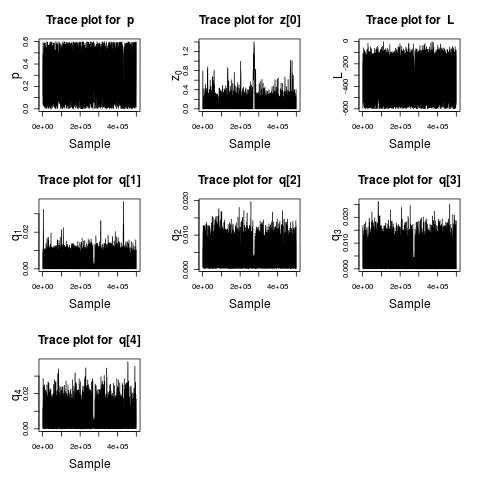
\includegraphics[scale=0.7]{./FigChap4/traces}
\caption{Trace plots for each of the  variables $\pars$ and $\q$.}
\label{figTraces}
\end{figure}

The marginal distribution of a random variable contains all the information about
that variable regardless of the value of other parameters. We are going
to use the marginals for each of the variables in the posterior distribution
in equation (\ref{eqnPosteriorFinal}) to obtain useful statistics about the 
parameters.
The histograms
for the   marginals  of each of the variables of interest in the posterior are shown
in Figure \ref{figHistograms}. 



%%%%%%%%%%%%%%%%%%%%%%%%%%%%%%%%%%%%%%%%%%%%%%%%%%This is the part I will probably have to change %%%%%%%%%%%%%%%%%%%%%%%%%%%%%%%%%%%%%%%%%%%



The next step for estimating the parameters is to decide what of the point estimates from equation (\ref{eqnpointestimates})
we will choose. By looking at Figure \ref{figHistograms},
it is clear that the  marginal posterior for the four sources is skewed and with a well-defined mode.
In this case, finding the maximum marginal posterior estimate is a reasonable choice. 
To find the  marginal maximum a posteriori estimate for  each of the four sources, it is
necessary to find
\begin{equation*}
\max_{q_{j}\in [0,\infty)}f(q_{j})\qquad\text{for } j=1,2,3,4,
\end{equation*}
where
\begin{equation*}
f(q_{j})=q_{j}^{\alpha_{j}-1}\exp(-\beta q_{j})\int \prod_{k\neq j}q_{k}^{\alpha_{k}-1}\exp(-\beta_{k}q_{k})
\exp\left(-\frac{1}{2\lambda^{2}}\|\widehat{A}\q-\y\|^{2}\right)dpdz_{0}dLd\tilde{\q}_{j},
\end{equation*}
where $d\tilde{\q}_{j}$ means the $j$-th term in the volume element $\prod_{k=1}^{4}dq_{k}$ has been suppressed.
Optimizing numerically $f$ is a challenging problem. 
First, the integral involved is high dimensional,
hence is necessary to use Monte Carlo integration to estimate it.  
The exponent in the integrand is a number close to zero
unless the term $\|\widehat{A}\q-\y\|^{2}=\mathcal{O}(10^{-12})$. 
Since Monte Carlo integration requires to evaluate the integrand
at a large and random number of different points in the domain of integration, we are going
to end up adding numbers that are, in general, smaller than the machine epsilon. 
Hence, numerically
the integrand will behave like a very small constant. The problem with this is that
all the information from the experimental data is contained in the integrand. So,
if the integrand behaves like a constant due to rounding error, the optimization
routine will not return an accurate value. Instead of using an optimization scheme, 
we will use the fact that the marginal 
posterior for the sources behaves similarly to a gamma distribution. In this case, we 
fit the gamma distribution that is closer to the marginal posterior and report
the statistics associated to that distribution. 
\\
For the parameters $\pars$ the situation is more subtle. For the parameter $p$
the distribution is unimodal. 
In this case we can choose the  mode as a point estimate.
The way to find the mode is by fitting a density over the histogram
of $p$ and pick the maximum of the fitting curve.
For the parameters $z_{0}$ and $L$, there is no distinctive point in
their distribution. In this case we pick a non-committal value like 
the median. The median of a one-dimensional probability density $\rho$ is defined
as the number $m^{*}$ such that 
\begin{equation*}
\int_{-\infty}^{m*}\rho(x)dx=\int_{m^{*}}^{\infty}\rho(x)dx=0.5.
\end{equation*}

In Figure \ref{figHistograms} it is shown the values of the point
estimates for each distribution and the fitting curves for the parametes $\pars$
and the sources $q_{1}$ to $q_{4}$.

\begin{figure}[H]
\centering
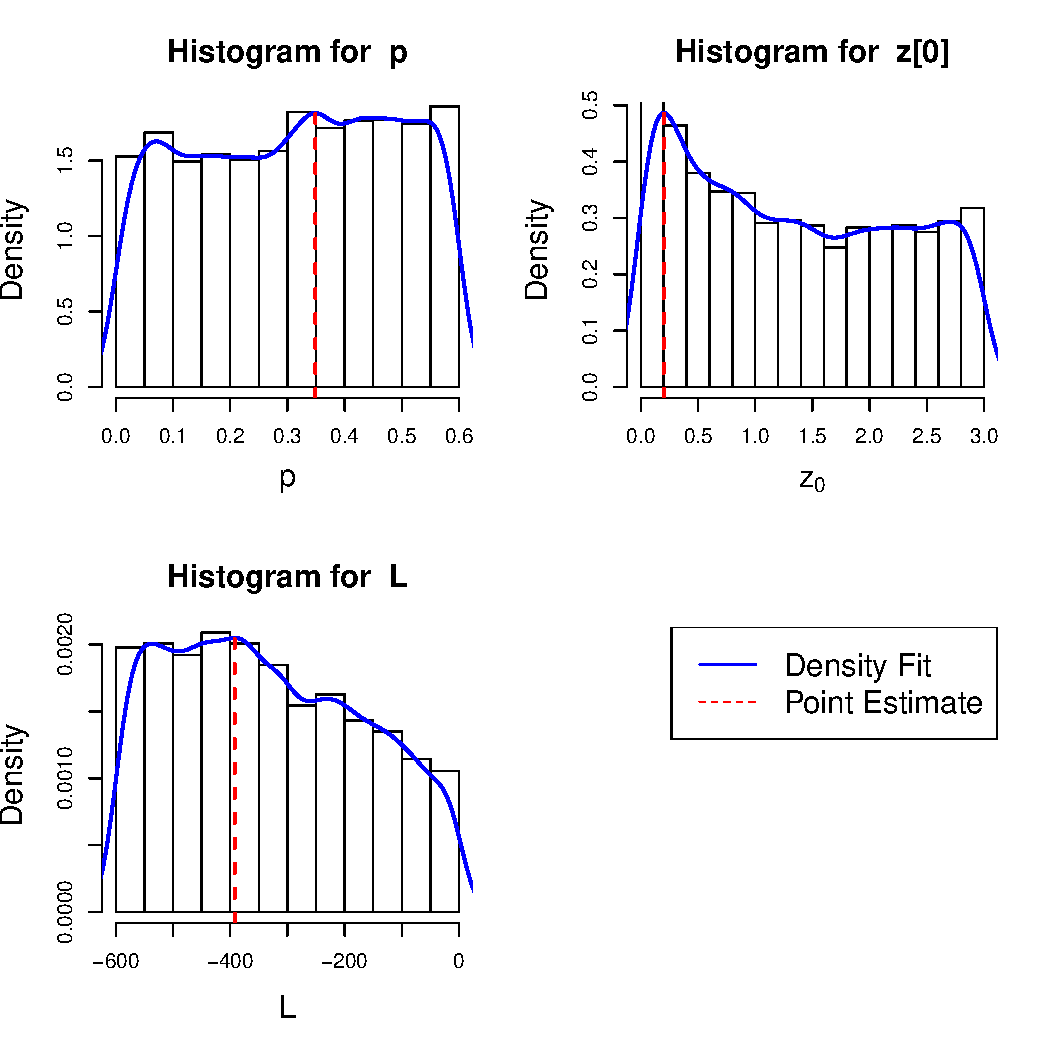
\includegraphics[scale=0.475]{./FigChap4/histogramsI}
%\caption{Histograms for the marginal distribution for each of the seven variables
%in the support of the posterior density.}
\label{figHistograms}
\end{figure}
\begin{figure}[H]
\centering
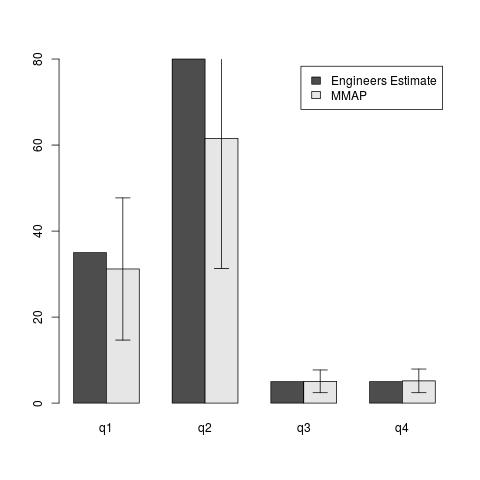
\includegraphics[scale=0.47]{./FigChap4/histogramsII}
\caption{Histograms for the marginal distribution for each of the seven variables
in the support of the posterior density in equation (\ref{eqnPosteriorFinal}).}
\label{figHistograms}
\end{figure}

For the uncertainty estimate, we pick the $68\%$ Bayesian confidence interval
for each of the parameters. Given a point estimate $x^{*}$ 
for a probability density $\rho$, a $68\%$ Bayesian confidence interval of that estimate, 
is defined as the ball of radius $r$ centered at $x^{*}$ such that
\begin{equation*}
\int_{B(x^{*},r)}\rho(x)dx=0.68,
\end{equation*} 

The estimates for the parameters and the uncertainties are shown in Table \ref{tabFinalEstimates}.

\begin{table}[H]
\centering
\begin{tabular}{|c|c|c|c|}
\hline 
Parameter & Point Estimate & Value & $68\%$ Confidence Interval\tabularnewline
\hline 
\hline 
$p$ & Mode & 0.3775 & $[0.2197,0.5352]$\tabularnewline
\hline 
$z_{0}$ & Median & 0.0886 & $[0.0024,0.1748]$\tabularnewline
\hline 
$L$ & Median & -357.60 & $[-651,11,-64.090]$\tabularnewline
\hline 
\end{tabular}
\caption{Parameters and their estimates and uncertainties. The sources are given in Tons per year.}
\label{tabFinalEstimates}
\end{table}


For the sources the results are shown in Figure 


\begin{figure}[H]
\centering
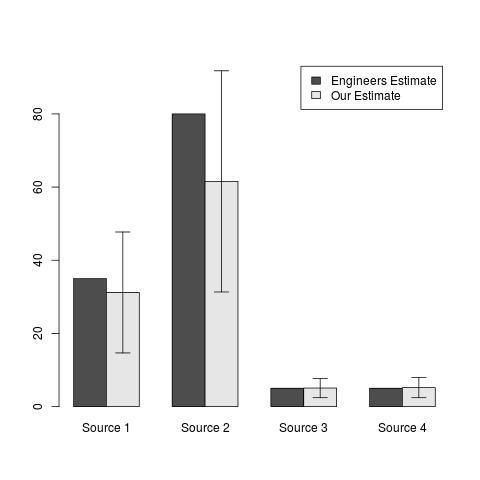
\includegraphics[scale=0.5]{./FigChap4/qUncertainty}
\caption{bla}
\label{figQUnicertainty}
\end{figure}
The results in Table \ref{tabFinalEstimates}, show that sources $3$ and $4$ are understimated by the engineers,
whereas sources $1$ and $2$ are overstimated. According to the engineer estimates, the smelter produces
125 tons per year. According to our results, this number is small  compared to the most likely value
of 181.407 tons per year. Another interesting result is that according to the literature,
the accepted ranges for the parameters $p$ and $L$ are $[0,0.4]$ and $[-500,1]$, respectively.
Our results show that these allowed ranges can be stretched in order for the model the explain
the experimental data available. 





\bibliography{Tesis}
\bibliographystyle{plain}
\end{document}
